%\nocite{273ba834}
%\nocite{53fd7d7e}
One of the most basic ideas in mathematics is that of an ordered pair of two sets say $a_{1}$ and $a_{2}$. We want to think of these two sets as a whole while rememebering which is the first and which is the second. So we cannot just take $\lbrace a_{1},a_{2} \rbrace$. It must be rather a mathematical object $(a_{1},a_{2})$ with the property that given another object of this form $(b_{1},b_{2})$ then we should have
\begin{align*}
  (a_{1},a_{2})
  =
  (b_{1},b_{2})
  \qquad
  &\Leftrightarrow
  \qquad
  \left(
    a_{1}
    =
    b_{1}
    \quad
    \land
    \quad
    a_{2}
    =
    b_{2}
  \right)
\end{align*}
This property can be viewed as a litmus test for being a good notion of ordered pair. In set theory ordered pairs must be sets. In TG the choice
\begin{align*}
  (a_{1},a_{2})
  :=
  (a_{1},a_{2})_{\textrm{k}}
  &:=
  \lbrace
    \lbrace
      a_{1}
    \rbrace,
    \lbrace
      a_{1},a_{2}
    \rbrace
  \rbrace
\end{align*}
is popular. But this choice is definitly not unique. For example we could also take
\begin{align*}
  (a,b)_{\textrm{w}}
  &:=
  \lbrace
    \lbrace
      \lbrace
        a
      \rbrace,
      \emptyset
    \rbrace,
    \lbrace
      \lbrace
        b
      \rbrace
    \rbrace
  \rbrace
\end{align*}
This will play a role in a moment. But we bind ourselves to the former here, as is usual in mathematics and has been the silently assumed convention in these notes.
\\
Restricting to a universe $\mathcal{U}$ let $\mathcal{U}_{\textrm{pair}}$ denote the set (of some larger universe) of all ordered pairs of sets in $\mathcal{U}$. Then we can define cartesian products. In what follows assume $Y_{1}$ and $Y_{2}$ as elements of $\mathcal{U}$. The cartesian product of $Y_{1}$ and $Y_{2}$ is defined by
\begin{align*}
  Y_{1}
  \times
  Y_{2}
  &:=
  \lbrace
      (y_{1},y_{2})
      \in
      \mathcal{U}_{\textrm{pair}}
    \,
    \vert
    \,
      y_{1}
      \in
      Y_{1}
      \quad
      \land
      \quad
      y_{2}
      \in
      Y_{2}
  \rbrace
\end{align*}
Further we have the two projection functions
\begin{align*}
  \mathrm{pr}_{1}
  \colon
  Y_{1}
  \times
  Y_{2}
  &\rightarrow
  Y_{1}
  \\
  (y_{1},y_{2})
  &\mapsto
  y_{1}
  \\\\
  \mathrm{pr}_{2}
  \colon
  Y_{1}
  \times
  Y_{2}
  &\rightarrow
  Y_{2}
  \\
  (y_{1},y_{2})
  &\mapsto
  y_{2}
\end{align*}
to the first and second coordinate, respectively. Note that a function
\begin{align*}
  f_{\times}
  \colon
  Y
  &\rightarrow
  Y_{1}
  \times
  Y_{2}
\end{align*}
is uniquely determined by functions $f_{1} \colon Y \rightarrow Y_{1}$ and $f_{2} \colon Y \rightarrow Y_{2}$ such that
\begin{align*}
  f_{1}
  &=
  \mathrm{pr}_{1}
  \circ
  f_{\times}
  \\
  f_{2}
  &=
  \mathrm{pr}_{2}
  \circ
  f_{\times}
\end{align*}
That is, for all $Y$ and all
\begin{align*}
  f_{1}
  \colon
  Y
  &\rightarrow
  Y_{1}
  \\
  f_{2}
  \colon
  Y
  &\rightarrow
  Y_{2}
\end{align*}
there is a unique function
\begin{align*}
  f_{\times}
  \colon
  Y
  &\rightarrow
  Y_{1}
  \times
  Y_{2}
\end{align*}
such that the diagram
\[
\begin{tikzcd}[sep=huge]
  &
  Y
  \arrow{dr}{f_{2}}
  \arrow{d}{f_{\times}}
  \arrow[swap]{d}{f_{\times}}
  \arrow[swap]{dl}{f_{1}}
  &
  \\
  Y_{1}
  &
  Y_{1}
  \times
  Y_{2}
  \arrow{r}{\mathrm{pr}_{2}}
  \arrow[swap]{l}{\mathrm{pr}_{1}}
  &
  Y_{2}
\end{tikzcd}
\]
commutes. Hence
\begin{align*}
  \left(
    Y_{1}
    \times
    Y_{2},
    \mathrm{pr}_{1},
    \mathrm{pr}_{2}
  \right)
\end{align*}
is a terminal object in the category $\pmb{\prod}(Y_{1},Y_{2})$ with objects $3$-tuples\footnote{note that these are recursively defined starting from ordered pairs} $(Y,f_{1},f_{2})$ as above and morphisms from $(Y,f_{1},f_{2})$ to $(Y^{\backprime},f_{1}^{\backprime},f_{2}^{\backprime})$ functions $h \colon Y \rightarrow Y^{\backprime}$ composed by function composition such that the diagram
\[
\begin{tikzcd}[sep=huge]
  &
  Y
  \arrow{dr}{f_{2}}
  \arrow{d}{h}
  \arrow[swap]{d}{h}
  \arrow[swap]{dl}{f_{1}}
  &
  \\
  Y_{1}
  &
  Y^{\backprime}
  \arrow{r}{f_{2}^{\backprime}}
  \arrow[swap]{l}{f_{1}^{\backprime}}
  &
  Y_{2}
\end{tikzcd}
\]
commutes. The terminal object of $\pmb{\prod}(Y_{1},Y_{2})$ is then called the \textbf{(binary) product (of $Y_{1}$ and $Y_{2}$)} while keeping the generalized {\glqq}the{\grqq} in mind. Namely defining the cartesian product $Y_{1} \times^{\textrm{w}} Y_{2}$ and projection functions $\mathrm{pr}_{1}^{\textrm{w}}$ and $\mathrm{pr}_{2}^{\textrm{w}}$ for $(a,b)_{\textrm{w}}$ in the same way as for $(a,b)_{\textrm{k}}$ we would find that also 
\begin{align*}
  \left(
    Y_{1}
    \times^{\textrm{w}}
    Y_{2},
    \mathrm{pr}_{1}^{\textrm{w}},
    \mathrm{pr}_{2}^{\textrm{w}}
  \right)
\end{align*}
is a terminal object in $\pmb{\prod}(Y_{1},Y_{2})$. So in a structural set theory one would rather try to define cartesian product by a universal property. Essentially one does so in ETCS and UFP-HoTT. In TG this knowledge also helps us since it does make sense to ask for binary products in this way w.r.t. to an arbitrary category and not just $\mathbf{Set}$. Though certainly not any category has all binary products.
\\
Now there is a certain way to specify subsets of the cartesian product. Namely by functions. A function $f \colon Y_{1} \rightarrow Y_{2}$ has a graph $\Gamma_{f}$ which is a subset of $Y_{1} \times Y_{2}$ and it is clear that for all $(y_{1},y_{2}) \in \Gamma_{f}$
\begin{align*}
  \left(
    f
    \circ
    \mathrm{pr}_{1}
  \right)
  (y_{1},y_{2})
  &=
  f(y_{1})
  =
  y_{2}
  =
  \mathrm{pr}_{2}
  (y_{1},y_{2})
\end{align*}
As a diagram, by allowing abuse of notation
\begin{align*}
  \mathrm{pr}_{i}
  &\doteq
  \mathrm{pr}_{i} \vert A
\end{align*}
for $A \subset Y_{1} \times Y_{2}$ and $i=1,2$, we then have
\[
\begin{tikzcd}[sep=large]
  &
  \Gamma_{f}
  \arrow{dr}{\mathrm{pr}_{2}}
  \arrow[swap]{dl}{\mathrm{pr}_{1}}
  &
  \\
  Y_{1}
  \arrow{rr}{f}
  &
  &
  Y_{2}
\end{tikzcd}
\]
If we further have another function $f^{\backprime} \colon Y_{1} \rightarrow Y_{2}$ then it is clear that for
\begin{align*}
  \mathrm{Eq}
  &:=
  \Gamma_{f}
  \cap
  \Gamma_{f^{\backprime}}
\end{align*}
we have
\[
\begin{tikzcd}[sep=large]
  &
  \mathrm{Eq}
  \arrow{dr}{\mathrm{pr}_{2}}
  \arrow[swap]{dl}{\mathrm{pr}_{1}}
  &
  \\
  Y_{1}
  \arrow{rr}{g}
  &
  &
  Y_{2}
\end{tikzcd}
\]
for $g \in \lbrace f,f^{\backprime} \rbrace$. The projection of $\mathrm{Eq}$ to the first coordinate is traditionally known as \textit{equalizer (of $f$ and $f^{\backprime}$)}. The equalizer of two functions is the part of the domain of the functions where they coincide. So $\mathrm{Eq}$ can be viewed as some kind of locus of $f$ and $f^{\backprime}$.
\\
Now actually we should take the universality of the product into account in order to make up for fixing a choice of ordered pair. This can be done by patching the respective diagrams together to get:
\begin{enumerate}
\item[(Eq)]
for each $3$-tuple $(Y,f_{1},f_{2})$ yielding a diagram as $(\mathrm{Eq},\mathrm{pr}_{1},\mathrm{pr}_{2})$ as above there is a unique function
\begin{align*}
  f_{\mathrm{Eq}}
  \colon
  Y
  &\rightarrow
  \mathrm{Eq}
\end{align*}
such that the diagram
\[
\begin{tikzcd}[sep=large]
  &
  Y
  \arrow{dddr}{f_{2}}
  \arrow{dd}{f_{\mathrm{Eq}}}
  \arrow[swap]{dd}{f_{\mathrm{Eq}}}
  \arrow[swap]{dddl}{f_{1}}
  &
  \\
  &
  &
  \\
  &
  \mathrm{Eq}
  \arrow[swap]{dr}{\mathrm{pr}_{2}}
  \arrow{dl}{\mathrm{pr}_{1}}
  &
  \\
  Y_{1}
  \arrow{rr}{g}
  &
  &
  Y_{2}
\end{tikzcd}
\]
commutes for all $g \in \lbrace f,f^{\backprime} \rbrace$
\end{enumerate}
Then we could potentially define a structural version of the equalizer in any category. But let us defer this for a while.
\\\\
We now look what we can abstract from these ideas. A very general form of
\[
\begin{tikzcd}[sep=large]
  &
  \mathrm{Eq}
  \arrow{dr}{\mathrm{pr}_{2}}
  \arrow[swap]{dl}{\mathrm{pr}_{1}}
  &
  \\
  Y_{1}
  \arrow{rr}{f}
  &
  &
  Y_{2}
\end{tikzcd}
\]
are cones. Assume a category $\mathbf{J}$ and a functor $F \colon \mathbf{J} \rightarrow \mathbf{C}$. Then define a function
\begin{align*}
  \mathsf{C}
  \colon
  \mathrm{ob}_{\mathbf{J}}
  &\rightarrow
  \mathrm{Mor}_{\mathbf{C}}
\end{align*}
with
\begin{align*}
  \mathsf{C}(J)
  &\in
  \mathrm{mor}_{\mathbf{C}}(X,F(J))
\end{align*}
for all $J$ to be a \textbf{cone (to $F$ with apex $X$)} if
\begin{enumerate}
\item[($\blacktriangle$)]
for all
\begin{align*}
  j_{12}
  &\in
  \mathrm{mor}_{\mathbf{J}}(J_{1},J_{2})
\end{align*}
the equation
\begin{align*}
  \mathsf{C}(J_{2})
  &=
  F(j_{12})
  \circ
  \mathsf{C}(J_{1})
\end{align*}
holds, that is, the diagram
\[
\begin{tikzcd}[sep=large]
  &
  X
  \arrow{dr}{\mathsf{C}(J_{2})}
  \arrow[swap]{dl}{\mathsf{C}(J_{1})}
  &
  \\
  F(J_{1})
  \arrow{rr}{F(j_{12})}
  &
  &
  F(J_{2})
\end{tikzcd}
\]
commutes
\end{enumerate}
Dually, a function
\begin{align*}
  \mathsf{C}^{\prime}
  \colon
  \mathrm{ob}_{\mathbf{J}}
  &\rightarrow
  \mathrm{Mor}_{\mathbf{C}}
\end{align*}
with
\begin{align*}
  \mathsf{C}^{\prime}(J)
  &\in
  \mathrm{mor}_{\mathbf{C}}(F(J),X)
\end{align*}
is a \textbf{cocone (to $F$ with apex $X$)} if
\begin{enumerate}
\item[($\blacktriangle^{\prime}$)]
for all
\begin{align*}
  j_{12}
  &\in
  \mathrm{mor}_{\mathbf{J}}(J_{1},J_{2})
\end{align*}
the equation
\begin{align*}
  \mathsf{C}^{\prime}(J_{1})
  &=
  \mathsf{C}^{\prime}(J_{2})
  \circ
  F(j_{12})
\end{align*}
holds, that is, the diagram
\[
\begin{tikzcd}[sep=large]
  F(J_{1})
  \arrow{rr}{F(j_{12})}
  \arrow[swap]{dr}{\mathsf{C}^{\prime}(J_{1})}
  &
  &
  F(J_{2})
  \arrow{dl}{\mathsf{C}^{\prime}(J_{2})}
  \\
  &
  X
  &
\end{tikzcd}
\]
commutes
\end{enumerate}
For a functor $F \colon \mathbf{J} \rightarrow \mathbf{C}$ let us define functors
\begin{align*}
  \mathrm{Cone}_{F}
  \colon
  \mathbf{C}^{\mathrm{op}}
  &\rightarrow
  \mathbf{Set}
  \\
  X
  &\mapsto
  \lbrace
      \mathsf{C}
      \colon
      \mathrm{ob}_{\mathbf{J}}
      \rightarrow
      \mathrm{Mor}_{\mathbf{C}}
    \,
    \vert
    \,
      \mathsf{C}
      \text{ is a cone to }
      F
      \text{ with apex }
      X
  \rbrace
  \\
  f_{12}^{\mathrm{op}}
  &\mapsto
  \left(
    \mathsf{C}
    \mapsto
    \left(
      J
      \mapsto
      \mathsf{C}(J)
      \circ
      f_{12}^{\mathrm{op}}
    \right)
  \right)
  \\
  \mathrm{Cone}_{F}^{\prime}
  \doteq
  \mathrm{Cocone}_{F}
  \colon
  \mathbf{C}
  &\rightarrow
  \mathbf{Set}
  \\
  X
  &\mapsto
  \lbrace
      \mathsf{C}^{\prime}
      \colon
      \mathrm{ob}_{\mathbf{J}}
      \rightarrow
      \mathrm{Mor}_{\mathbf{C}}
    \,
    \vert
    \,
      \mathsf{C}^{\prime}
      \text{ is a cocone to }
      F
      \text{ with apex }
      X
  \rbrace
  \\
  f_{12}
  &\mapsto
  \left(
    \mathsf{C}^{\prime}
    \mapsto
    \left(
      J
      \mapsto
      f_{12}
      \circ
      \mathsf{C}^{\prime}(J)
    \right)
  \right)
\end{align*}
Call $\mathrm{Cone}_{F}(X)$ the \textbf{(set of) cones (to $F$ with apex $X$)} and dually $\mathrm{Cocone}_{F}(X)$ the \textbf{(set of) cocones (to $F$ with apex $X$)}. Given a cone $\mathsf{C} \in \mathrm{Cone}_{F}(X)$ we call $\mathsf{C}(J)$ the \textbf{$J$-th leg (of $\mathsf{C}$)} while given a cocone $\mathsf{C}^{\prime} \in \mathrm{Cocone}_{F}(X)$ we call $\mathsf{C}^{\prime}(J)$ the \textbf{$J$-th coleg (of $\mathsf{C}^{\prime}$)}.
\\
With this terminology as backbone we can easily generalize the property (Eq) from above by the following definitions.
\begin{enumerate}
\item[(U${}_{\blacktriangle}$)]
A cone $\mathsf{C}_{T}$ is called \textbf{limiting cone (to $F$ with apex $X_{T}$)} if for any cone $\mathsf{C}$ to $F$ with apex $X$ there is precisely one morphism
\begin{align*}
  f
  &\in
  \mathrm{mor}_{\mathbf{C}}(X,X_{T})
\end{align*}
such that for all $J$ the equation
\begin{align*}
  \mathsf{C}(J)
  &=
  \mathsf{C}_{T}(J)
  \circ
  f
\end{align*}
holds, that is, the diagram
\[
\begin{tikzcd}[sep=large]
  &
  X
  \arrow{d}{f}
  \arrow[swap]{ddl}{\mathsf{C}(J)}
  \\
  &
  X_{T}
  \arrow{dl}{\mathsf{C}_{T}(J)}
  \\
  F(J)
\end{tikzcd}
\]
commutes. $(X_{T},F,\mathsf{C}_{T})$ is called \textbf{limit of $F$} if $\mathsf{C}_{T}$ is a limiting cone to $F$ with apex $X_{T}$.
\item[(U${}_{\blacktriangle^{\prime}}$)]
A cocone $\mathsf{C}_{I}^{\prime}$ for $F$ is called \textbf{colimiting cocone (to $F$ with apex $X_{I}$)} if for any cocone $\mathsf{C}^{\prime}$ to $F$ with apex $X$ there is precisely one morphism
\begin{align*}
  f
  &\in
  \mathrm{mor}_{\mathbf{C}}(X_{I},X)
\end{align*}
such that for all $J$ the equation
\begin{align*}
  \mathsf{C}^{\prime}(J)
  &=
  f
  \circ
  \mathsf{C}_{I}^{\prime}(J)
\end{align*}
holds, that is, the diagram
\[
\begin{tikzcd}[sep=large]
  F(J)
  \arrow{dr}{\mathsf{C}_{I}^{\prime}(J)}
  \arrow[swap]{ddr}{\mathsf{C}^{\prime}(J)}
  &
  \\
  &
  X_{I}
  \arrow{d}{f}
  \\
  &
  X
\end{tikzcd}
\]
commutes. $(F,X_{I},\mathsf{C}_{I}^{\prime})$ is called \textbf{colimit of $F$} if $\mathsf{C}_{I}^{\prime}$ is a colimiting cocone to $F$ with apex $X_{I}$.
\end{enumerate}
For $(X_{T},F,\mathsf{C}_{T})$ to be a limit of $F$ means that for all cones $\mathsf{C}$ to $F$ with apex $X$ and all $J_{1},J_{2},j_{12}$ there is exactly one morphism
\begin{align*}
  f
  &\in
  \mathrm{mor}_{\mathbf{C}}(X,X_{T})
\end{align*}
such that the diagram
\[
\begin{tikzcd}[sep=huge]
  &
  X
  \arrow{dddr}{\mathsf{C}(J_{2})}
  \arrow{dd}{f}
  \arrow[swap]{dd}{f}
  \arrow[swap]{dddl}{\mathsf{C}(J_{1})}
  &
  \\
  &
  &
  \\
  &
  X_{T}
  \arrow[swap]{dr}{\mathsf{C}_{T}(J_{2})}
  \arrow{dl}{\mathsf{C}_{T}(J_{1})}
  &
  \\
  F(J_{1})
  \arrow{rr}{F(j_{12})}
  &
  &
  F(J_{2})
\end{tikzcd}
\]
commutes. With some identities the diagram can be expanded to
\[
\begin{tikzcd}[sep=huge]
  X
  \arrow{rrr}{f}
  \arrow[swap]{dr}{\mathrm{id}_{X}}
  \arrow[swap]{ddd}{\mathsf{C}(J_{1})}
  &
  &
  &
  X_{T}
  \arrow{ddd}{\mathsf{C}_{T}(J_{1})}
  \arrow{dl}{\mathrm{id}_{X_{T}}}
  \\
  &
  X
  \arrow{r}{f}
  \arrow[swap]{d}{\mathsf{C}(J_{2})}
  &
  X_{T}
  \arrow{d}{\mathsf{C}_{T}(J_{2})}
  &
  \\
  &
  F(J_{2})
  \arrow{r}{\mathrm{id}_{F}(J_{2})}
  &
  F(J_{2})
  &
  \\
  F(J_{1})
  \arrow{rrr}{\mathrm{id}_{F}(J_{1})}
  \arrow{ur}{F(j_{12})}
  &
  &
  &
  F(J_{1})
  \arrow[swap]{ul}{F(j_{12})}
\end{tikzcd}
\]
and one might wonder if there is a functor such that $\mathsf{C}_{T}$ and $\mathsf{C}$ become natural transformations from this functor to $F$ since cones seem very close to such a thing? But this is accomplished by the constant functor $\mathrm{C}_{X_{T}} \colon \mathbf{J} \rightarrow \mathbf{C}$ with target $X$ and the constant functor $\mathrm{C}_{X} \colon \mathbf{J} \rightarrow \mathbf{C}$ with target $X$, respectively. So we get
\[
\begin{tikzcd}[sep=huge]
  \mathrm{C}_{X}(J_{1})
  \arrow{rrr}{f}
  \arrow[swap]{dr}{\mathrm{C}_{X}(j_{12})}
  \arrow[swap]{ddd}{\mathsf{C}(J_{1})}
  &
  &
  &
  \mathrm{C}_{X_{T}}(J_{1})
  \arrow{ddd}{\mathsf{C}_{T}(J_{1})}
  \arrow{dl}{\mathrm{C}_{X_{T}}(j_{12})}
  \\
  &
  \mathrm{C}_{X}(J_{2})
  \arrow{r}{f}
  \arrow[swap]{d}{\mathsf{C}(J_{2})}
  &
  \mathrm{C}_{X_{T}}(J_{2})
  \arrow{d}{\mathsf{C}_{T}(J_{2})}
  &
  \\
  &
  F(J_{2})
  \arrow{r}{\mathrm{id}_{F}(J_{2})}
  &
  F(J_{2})
  &
  \\
  F(J_{1})
  \arrow{rrr}{\mathrm{id}_{F}(J_{1})}
  \arrow{ur}{F(j_{12})}
  &
  &
  &
  F(J_{1})
  \arrow[swap]{ul}{F(j_{12})}
\end{tikzcd}
\]
Now observe that the bottom square of the box is a natural transformation from $F$ to $F$. But what about the top square? Well, yes. Just define natural transformations
\begin{align*}
  \Delta_{\mathbf{C}}(f_{12})
  \colon
  \mathrm{C}_{X_{1}}
  &\Rightarrow
  \mathrm{C}_{X_{2}}
  \\
  J
  &\mapsto
  f_{12}
\end{align*}
and use $\Delta_{\mathbf{C}}(f)$. Thus the commutativity of one of the last three equivalent diagrams for all $J_{1},J_{2},j_{12}$ is equivalent to the commutativity of the diagram
\[
\begin{tikzcd}[sep=large]
  \mathrm{C}_{X}
  \arrow{r}{\Delta_{\mathbf{C}}(f)}
  \arrow[swap]{d}{\mathsf{C}}
  &
  \mathrm{C}_{X_{T}}
  \arrow{d}{\mathsf{C}_{T}}
  \\
  F
  \arrow{r}{\mathrm{id}_{F}}
  &
  F
\end{tikzcd}
\]
in $\mathbf{C}^{\mathbf{J}}$. But this looks like a morphism diagram of some comma category. This comma category has a nice depiction using the functor
\begin{align*}
  \Delta_{\mathbf{C}}
  \colon
  \mathbf{C}
  &\rightarrow
  \mathbf{C}^{\mathbf{J}}
  \\
  X
  &\mapsto
  \mathrm{C}_{X}
  \\
  f_{12}
  &\mapsto
  \Delta_{\mathbf{C}}(f_{12})
\end{align*}
$\Delta_{\mathbf{C}}$ is called the \textbf{diagonal functor (w.r.t. $\mathbf{J}$)}. With this depiction a limit of $F$ is then nothing but a terminal object in $(\Delta_{\mathbf{C}} \downarrow \mathrm{c}_{F})$ and hence by theorem \ref{thm:unimorequivuni} this is to say that
\begin{align*}
  \mathsf{C}_{T}
  \in
  \mathrm{mor}_{\mathbf{C}^{\mathbf{J}}}(\Delta_{\mathbf{C}}(X_{T}),F)
\end{align*}
is a $\Delta_{\mathbf{C}}$-terminal morphism for $F$.
\\\\
After all, we have shown that
\\
\begin{thm}
\label{thm:limitequiv}
\begin{enumerate}
\item[(1T)]
$(X_{T},F,\mathsf{C}_{T})$ is a limit of $F$ if and only if
\begin{align*}
  \mathsf{C}_{T}
  \in
  \mathrm{mor}_{\mathbf{C}^{\mathbf{J}}}(\Delta_{\mathbf{C}}(X_{T}),F)
\end{align*}
is a $\Delta_{\mathbf{C}}$-terminal morphism for $F$.
\item[(1I)]
$(F,X_{I},\mathsf{C}_{I}^{\prime})$ is a colimit of $F$ if and only if
\begin{align*}
  \mathsf{C}_{I}^{\prime}
  \in
  \mathrm{mor}_{\mathbf{C}^{\mathbf{J}}}(F,\Delta_{\mathbf{C}}(X_{I}))
\end{align*}
is a $\Delta_{\mathbf{C}}$-initial morphism for $F$.
\end{enumerate}
\end{thm}
\begin{prf}
\begin{enumerate}
\item[(1T)]
See the discussion above.
\item[(1I)]
The duality principle \ref{thm:dp}.
\end{enumerate}
\phantom{proven}
\hfill
$\square$
\end{prf}
For the sake of completeness let us write down the commutative diagram for colimiting cocones $\mathsf{C}_{I}^{\prime}$:
\[
\begin{tikzcd}[sep=huge]
  F(J_{1})
  \arrow{rr}{F(j_{12})}
  \arrow{dr}{\mathsf{C}_{I}^{\prime}(J_{1})}
  \arrow[swap]{dddr}{\mathsf{C}^{\prime}(J_{1})}
  &
  &
  F(J_{2})
  \arrow{dddl}{\mathsf{C}^{\prime}(J_{2})}
  \arrow[swap]{dl}{\mathsf{C}_{I}^{\prime}(J_{2})}
  \\
  &
  X_{I}
  \arrow{dd}{f}
  \arrow[swap]{dd}{f}
  &
  \\
  \\
  &
  X
  &
\end{tikzcd}
\]
Now theorem \ref{thm:limitequiv} shows that limits and colimits are special cases of universality. But note that terminal and initial objects of $\mathbf{C}$ are limits and colimits, respectively, of a functor $F \colon \varnothing \rightarrow \mathbf{C}$. By the way, for a functor $F \colon \mathbf{J} \rightarrow \mathbf{C}$ universal objects of the index category $\mathbf{J}$ can be used to compute apices of a colimiting cone and limiting cone, respectively. This is the next theorem.
\\
\begin{thm}
\label{thm:limonuniob}
Given a functor $F \colon \mathbf{J} \rightarrow \mathbf{C}$ such that
\begin{enumerate}
\item[(1T)]
$\mathbf{J}$ has a terminal object. If $j$ denotes the unique arrow from $J$ to $1_{\mathbf{J}}$ then mapping $J$ to $F(j)$ denoted $\mathsf{C}_{I}^{\prime}$ is a colimit cocone to $F$ with apex $F(1_{\mathbf{J}})$.
\item[(1I)]
$\mathbf{J}$ has an initial object. If $j$ denotes the unique arrow from $0_{\mathbf{J}}$ to $J$ then mapping $J$ to $F(j)$ denoted $\mathsf{C}_{T}$ is a limit cone to $F$ with apex $F(0_{\mathbf{J}})$.
\end{enumerate}
\end{thm}
\begin{prf}
\begin{enumerate}
\item[(1T)]
Let's proceed in two steps and first show that $\mathsf{C}_{I}^{\prime}$ is a cocone before proving it to be colimiting.
\begin{description}
\item[Step 1]
This is clear since for all $J_{1},J_{2},j_{12}$ we have
\begin{align*}
  \mathsf{C}_{I}^{\prime}(J_{2})
  \circ
  F(j_{12})
  &=
  F(j_{2})
  \circ
  F(j_{12})
  =
  F(j_{2} \circ j_{12})
  =
  F(j_{1})
\end{align*}
if $j_{k}$ denote the unique morphisms from $J_{k}$ to $1_{\mathbf{J}}$ for $k = 1,2$.
\item[Step 2]
If $\mathsf{C}^{\prime}$ denotes any cocone to $F$ with apex $X$ then if there further is a morphism
\begin{align*}
  f
  \in
  \mathrm{mor}_{\mathbf{C}}
  \left(
    F(1_{\mathbf{J}})
    ,
    X
  \right)
\end{align*}
such that
\begin{align*}
  f
  \circ
  \mathsf{C}_{I}^{\prime}(J)
  &=
  \mathsf{C}^{\prime}(J)
\end{align*}
for all $J$ it must be $\mathsf{C}^{\prime}(1_{\mathbf{J}})$ as can be seen from the case $J = 1_{\mathbf{J}}$. But then we have
\begin{align*}
  f
  \circ
  \mathsf{C}_{I}^{\prime}(J)
  &=
  \mathsf{C}^{\prime}(1_{\mathbf{J}})
  \circ
  \mathsf{C}_{I}^{\prime}(J)
  =
  \mathsf{C}^{\prime}(1_{\mathbf{J}})
  \circ
  F(j)
  =
  \mathsf{C}^{\prime}(J)
\end{align*}
for all $J$ where $j$ is the unique morphism from $J$ to $1_{\mathbf{J}}$.
\end{description}
\item[(1I)]
The duality principle \ref{thm:dp}.
\end{enumerate}
\phantom{proven}
\hfill
$\square$
\end{prf}
The statement is even better than just computing apices since it proves the existence of limits and colimits in some (unfortunately not so relevant) cases. It is, in fact, an important question which limits and colimits of functors with fixed codomain categories exist and it will accompany us during this subsection.
\\\\
Having established the different characterizations of limits and colimits we turn to the special cases of them which are well-known in mathematics. Though not necessarily as categorical concepts. Hence the following example.
\\
\begin{exa}
\label{exa:oflimits}
This example is built up as follows. We go through a list of interesting possibilities what $\mathbf{J}$ can stand for and define names for the according colimits and limits of functors $F \colon \mathbf{J} \rightarrow \mathbf{C}$ and $P \colon \mathbf{J}^{\mathrm{op}} \rightarrow \mathbf{C}$, respectively. In some cases we will go in greater detail for $\mathbf{C} = \mathbf{Set}$ or whatever seems interesting. Moreover we sometimes visualize $\mathbf{J}$ by a diagram consisting of all arrows.\footnote{note that objects are the identity arrows} So let $F \colon \mathbf{J} \rightarrow \mathbf{C}$ and $P \colon \mathbf{J}^{\mathrm{op}} \rightarrow \mathbf{C}$ denote functors.
\begin{enumerate}
\item[(1)]
Let $\mathbf{J}$ be category with finite object set. Then limits of $P$ and colimits of $F$ are called \textbf{finite}.
\item[(2)]
Let $\mathbf{J}$ be discrete. A limit of $P$ is a \textbf{product (in $\mathbf{C}$)}. Dually, a colimit of $F$ is a \textbf{coproduct (in $\mathbf{C}$)}. If addtionally $\mathbf{J}$ has exactly two objects $Z_{1}$ and $Z_{2}$ then a limit of $P$ is a \textbf{binary product (in $\mathbf{C}$)} while a colimit of $F$ is a \textbf{binary coproduct (in $\mathbf{C}$)}. If $(\mathrm{Pr},P,\mathsf{Pr})$ is a product it is common to write
\begin{align*}
  \prod_{J \in \mathrm{ob}_{\mathbf{J}}}
  P(J)
  \doteq
  \prod_{J \in \mathrm{ob}_{\mathbf{J}}}^{\mathbf{C}}
  P(J)
  &:=
  \mathrm{Pr}
\end{align*}
and
\begin{align*}
  \mathrm{pr}_{J}
  \doteq
  \mathrm{pr}_{J}^{\mathbf{C}}
  &:=
  \mathsf{Pr}(J)
\end{align*}
while in the case of binary products one also writes
\begin{align*}
  P(Z_{1})
  \times
  P(Z_{2})
  \doteq
  P(Z_{1})
  \times_{\mathbf{C}}
  P(Z_{2})
  &:=
  \mathrm{Pr}
\end{align*}
Dually, if $(F,\mathrm{Pr}^{\prime},\mathsf{I})$ is a coproduct it is common to write
\begin{align*}
  \coprod_{J \in \mathrm{ob}_{\mathbf{J}}}
  F(J)
  \doteq
  \coprod_{J \in \mathrm{ob}_{\mathbf{J}}}^{\mathbf{C}}
  F(J)
  &:=
  \mathrm{Pr}^{\prime}
\end{align*}
and
\begin{align*}
  \mathrm{i}_{J}
  \doteq
  \mathrm{i}_{J}^{\mathbf{C}}
  &:=
  \mathsf{I}(J)
\end{align*}
while in the case of binary coproducts one also writes
\begin{align*}
  F(Z_{1})
  \sqcup
  F(Z_{2})
  \doteq
  F(Z_{1})
  \sqcup_{\mathbf{C}}
  F(Z_{2})
  &:=
  \mathrm{Pr}^{\prime}
\end{align*}
For $\mathbf{C} = \mathbf{Set}$ the binary products are precisely the cartesian products as described at the beginning of the subsection. Reversing all arrows there would quite directly show that binary coproducts are precisely the disjoint union of two sets. More generally, one can show that products and coproducts precisely are cartesians products and disjoint unions, respectively, of arbitrary families of sets. Hence in $\mathbf{Set}$ all products and coproducts exist. There is an interesting point here regarding the dependent products and sums we mentioned in the introduction to this section \ref{sec:uni}. Namely, the dependent product in $\mathbf{Set}$ is the product in $\mathbf{Set}$ while the dependent sum in $\mathbf{Set}$ is the coproduct in $\mathbf{Set}$. But in general the dependent cases are something else. They are still something like products and coproducts: they are not indexed by a set but an object of the category of discourse.\footnote{see the according \cite{wiki-nlab0000} articles for more on this} Anyways, the product
\begin{align*}
  \prod_{J \in \mathrm{ob}_{\mathbf{J}}}^{\mathbf{Set}}
  P(J)
\end{align*}
is usually taken as the set of functions $f \colon \mathrm{ob}_{\mathbf{J}} \rightarrow \bigcup_{\mathrm{ob}_{\mathbf{J}}}P(J)$ such that $f(J) \in P(J)$ for all $J$. We confine ourselves to this convention and hence
\begin{align*}
  f
  &\in
  \prod_{J \in \mathrm{ob}_{\mathbf{J}}}^{\mathbf{Set}}
  P(J)
\end{align*}
is called \textbf{dependent function (through $P$)}. To define a dependent function we write
\begin{align*}
  f
  :=
  \left(
    J
    \mapsto
    f(J)
  \right)
  &\colon
  \prod_{J \in \mathrm{ob}_{\mathbf{J}}}^{\mathbf{Set}}
  P(J)
\end{align*}
(as in UFP-HoTT).
\item[(3)]
Let $\mathbf{J}$ be a category such that its set of objects contains exactly two elements - one named $Z_{1}$ the other $Z_{2}$ - and such that the only non-identity morphisms are the exactly two elements $z,z^{\backprime}$ of $\mathrm{mor}_{\mathbf{J}}(Z_{2},Z_{1})$. As a diagram this category can be visualized as
\[
\begin{tikzcd}[sep=huge]
  Z_{2}
  \arrow[shift left=0.5ex]{r}{z}
  \arrow[swap,shift right=0.5ex]{r}{z^{\backprime}}
  &
  Z_{1}
\end{tikzcd}
\]
A limit of $P$ is an \textbf{equalizer (in $\mathbf{C}$)} while dually a colimit of $F$ is a \textbf{coequalizer (in $\mathbf{C}$)}. $(\mathrm{Eq},P,\mathsf{Eq})$ being an equalizer of $P$ means that for all
\begin{align*}
  z_{12}^{\mathrm{op}}
  \in
  \mathrm{mor}_{\mathbf{J}}(Z_{2},Z_{1})
\end{align*}
and $\mathsf{C}$ any cone to $P$ with apex $X$ there is precisely one arrow
\begin{align*}
  f
  &\in
  \mathrm{mor}_{\mathbf{C}}(X,\mathrm{Eq})
\end{align*}
such that the diagram
\[
\begin{tikzcd}[sep=huge]
  &
  X
  \arrow{dddr}{\mathsf{C}(Z_{2})}
  \arrow{dd}{f}
  \arrow[swap]{dd}{f}
  \arrow[swap]{dddl}{\mathsf{C}(Z_{1})}
  &
  \\
  &
  &
  \\
  &
  \mathrm{Eq}
  \arrow[swap]{dr}{\mathsf{Eq}(Z_{2})}
  \arrow{dl}{\mathsf{Eq}(Z_{1})}
  &
  \\
  P(Z_{1})
  \arrow{rr}{P(z_{12}^{\mathrm{op}})}
  &
  &
  P(Z_{2})
\end{tikzcd}
\]
commutes. But this is to say that given $\mathrm{Eq} \in \mathrm{ob}_{\mathbf{C}}$ and
\begin{align*}
  \mathsf{Eq}(Z_{1})
  \in
  \mathrm{mor}_{\mathbf{C}}(\mathrm{Eq},F(Z_{1}))
\end{align*}
such that
\begin{align*}
  P(z)
  \circ
  \mathsf{Eq}(Z_{1})
  &=
  P(z^{\backprime})
  \circ
  \mathsf{Eq}(Z_{1})
\end{align*}
then for any $X \in \mathrm{ob}_{\mathbf{C}}$ and
\begin{align*}
  \mathsf{C}(Z_{1})
  \in
  \mathrm{mor}_{\mathbf{C}}(X,P(Z_{1}))
\end{align*}
such that
\begin{align*}
  P(z)
  \circ
  \mathsf{C}(Z_{1})
  &=
  P(z^{\backprime})
  \circ
  \mathsf{C}(Z_{1})
\end{align*}
there is precisely one arrow
\begin{align*}
  f
  &\in
  \mathrm{mor}_{\mathbf{C}}(X,\mathrm{Eq})
\end{align*}
such that
\begin{align*}
  \mathsf{C}(Z_{1})
  &=
  \mathsf{Eq}(Z_{1})
  \circ
  f
\end{align*}
that is, the diagram
\[
\begin{tikzcd}[sep=huge]
  \mathrm{Eq}
  \arrow{r}{\mathsf{Eq}(Z_{1})}
  &
  P(Z_{1})
  \arrow[shift left=0.5ex]{r}{P(z)}
  \arrow[swap,shift right=0.5ex]{r}{P(z^{\backprime})}
  &
  P(Z_{2})
  \\
  X
  \arrow{u}{f}
  \arrow[swap]{ur}{\mathsf{C}(Z_{1})}
  &
  &
\end{tikzcd}
\]
commutes. This is why people often say a bit sloppy that
\begin{align*}
  \mathrm{Eq}
  &\doteq
  (\mathrm{Eq},\mathsf{Eq}(Z_{1}))
\end{align*}
is the equalizer of $P(z)$ and $P(z^{\backprime})$. And the same works dually for the coequalizer with the commutative diagram
\[
\begin{tikzcd}[sep=huge]
  F(Z_{2})
  \arrow[shift left=0.5ex]{r}{F(z)}
  \arrow[swap,shift right=0.5ex]{r}{F(z^{\backprime})}
  &
  F(Z_{1})
  \arrow{r}{\mathsf{Eq}^{\prime}(Z_{1})}
  \arrow[swap]{dr}{\mathsf{C}^{\prime}(Z_{1})}
  &
  \mathrm{Eq}^{\prime}
  \arrow{d}{f}
  \\
  &
  &
  X
\end{tikzcd}
\]
and the same sloppy convention. For the case $\mathbf{C} = \mathbf{Set}$ we already treated the equalizer above as essentially being the subset of the domain (namely $\mathrm{Eq}$) on which functions $f,f^{\backprime} \colon Y_{1} \rightarrow Y_{2}$ agree. The case of the coequalizer is no less worthwhile. The coequalizer of $f,f^{\backprime} \colon Y_{1} \rightarrow Y_{2}$ would be $\mathrm{Eq}^{\prime} = Y_{2} \slash \sim$ where $\sim$ is the smallest equivalence relation for which
\begin{align*}
  f(y_{1})
  &\sim
  f^{\backprime}(y_{1})
\end{align*}
is true for all $y_{1} \in Y_{1}$. $\mathsf{Eq}^{\prime}(Z_{1})$ is then clearly the the projection which maps $y_{2}$ to its equivalence class under $\sim$. Note that in $\mathbf{Set}$ all equalizers and coequalizers exist.
\item[(4)]
Let $\mathbf{J}$ be a category such that its set of objects contains exactly three elements - one named $Z_{1}$, one $Z_{2}$ and the third $Z$. Further we require that the only non-identity morphisms are the exactly one element $z_{1}$ of $\mathrm{mor}_{\mathbf{J}}(Z,Z_{1})$ and the exactly one element $z_{2}$ of $\mathrm{mor}_{\mathbf{J}}(Z,Z_{2})$. This is visualized by the roof or span
\[
\begin{tikzcd}[sep=huge]
  &
  Z
  \arrow[swap]{dl}{z_{1}}
  \arrow{dr}{z_{2}}
  &
  \\
  Z_{1}
  &
  &
  Z_{2}
\end{tikzcd}
\]
as some authors say. A limit of $P$ is a \textbf{pullback (in $\mathbf{C}$)} or equivalently \textbf{fibered product (in $\mathbf{C}$)} while dually a colimit of $F$ is a \textbf{pushout (in $\mathbf{C}$)} or equivalently \textbf{fibered/amalgamated coproduct (in $\mathbf{C}$)}. $(\mathrm{Pb},P,\mathsf{Pr})$ being a pullback means that for any cone $\mathsf{C}$ to $P$ with apex $X$ there are unique morphisms
\begin{align*}
  f_{1}
  &\in
  \mathrm{mor}_{\mathbf{C}}(X,\mathrm{Pb})
  \\
  f_{2}
  &\in
  \mathrm{mor}_{\mathbf{C}}(X,\mathrm{Pb})
\end{align*}
such that the diagram
\[
\begin{tikzcd}[sep=huge]
  X
  \arrow[bend left=30]{drrr}{\mathsf{C}(Z_{2})}
  \arrow[shift left=1ex,shorten >= 1em]{dr}{f_{2}}
  \arrow[dash,pos=0.95]{dr}{\mathsf{C}(Z)}
  \arrow[swap,shift right=1ex,shorten >= 1em]{dr}{f_{1}}
  \arrow[swap,bend right=30]{dddr}{\mathsf{C}(Z_{1})}
  &
  &
  &
  \\
  &
  \mathrm{Pb}
  \arrow{rr}{\mathsf{Pr}(Z_{2})}
  \arrow[shift left=1ex,shorten <= 2em]{ddrr}{\mathsf{Pr}(Z)}
  \arrow[swap,pos=0.1]{ddrr}{\mathsf{C}(Z)}
  \arrow[swap,shift right=1ex,shorten <= 2em]{ddrr}{\mathsf{Pr}(Z)}
  \arrow[swap]{dd}{\mathsf{Pr}(Z_{1})}
  &
  &
  P(Z_{2})
  \arrow{dd}{P(z_{2})}
  \\
  &
  &
  &
  \\
  &
  P(Z_{1})
  \arrow{rr}{P(z_{1})}
  &
  &
  P(Z)
\end{tikzcd}
\]
commutes. This can be seen by patching the respective limit diagrams for $z_{1}$ and $z_{2}$ together. Since $f_{1}$ is unique we have $f_{1} = f_{2}$.\footnote{symmetrically we can derive that by the uniquenes of $f_{2}$} Hence $(\mathrm{Pb},P,\mathsf{Pr})$ is a pullback if and only if for any cone $\mathsf{C}$ to $P$ with apex $X$ there is a unique morphism
\begin{align*}
  f
  &\in
  \mathrm{mor}_{\mathbf{C}}(X,\mathrm{Pb})
\end{align*}
such that the diagram
\[
\begin{tikzcd}[sep=huge]
  X
  \arrow[bend left=30]{drr}{\mathsf{C}(Z_{2})}
  \arrow{dr}{f}
  \arrow[swap,bend right=30]{ddr}{\mathsf{C}(Z_{1})}
  &
  &
  &
  \\
  &
  \mathrm{Pb}
  \arrow{r}{\mathsf{Pr}(Z_{2})}
  \arrow[swap]{d}{\mathsf{Pr}(Z_{1})}
  &
  P(Z_{2})
  \arrow{d}{P(z_{2})}
  \\
  &
  P(Z_{1})
  \arrow{r}{P(z_{1})}
  &
  P(Z)
\end{tikzcd}
\]
commutes. It is common to write
\begin{align*}
  P(Z_{1})
  \times_{P(Z)}
  P(Z_{2})
  &:=
  \mathrm{Pb}
  \\
  \mathrm{Pr}_{1}
  &:=
  \mathsf{Pr}(Z_{1})
  \\
  \mathrm{Pr}_{2}
  &:=
  \mathsf{Pr}(Z_{2})
\end{align*}
and say a bit sloppy that
\begin{align*}
  P(Z_{1})
  \times_{P(Z)}
  P(Z_{2})
  &\doteq
  \left(
    P(Z_{1})
    \times_{P(Z)}
    P(Z_{2}),
    \mathrm{Pr}_{1},
    \mathrm{Pr}_{2}
  \right)
\end{align*}
is the pullback of $P(z_{1})$ and $P(z_{2})$. For some cases of $\mathbf{C}$, especially when any kind of bundles play a role, one also says that
\begin{align*}
  P(z_{1})^{\ast}(P(z_{2}))
  &\doteq
  \mathrm{Pr}_{1}
\end{align*}
is the pullback of $P(z_{2})$ along $P(z_{1})$ or symmetrically that
\begin{align*}
  P(z_{2})^{\ast}(P(z_{1}))
  &\doteq
  \mathrm{Pr}_{2}
\end{align*}
is the pullback of $P(z_{1})$ along $P(z_{2})$. Dually, $(F,\mathrm{Po},\mathsf{I})$ is a pushout if and only if for any cocone $\mathsf{C}$ to $F$ with apex $X$ there is a unique morphism
\begin{align*}
  f
  &\in
  \mathrm{mor}_{\mathbf{C}}(\mathrm{Po},X)
\end{align*}
such that the diagram
\[
\begin{tikzcd}[sep=huge]
  X
  &
  &
  &
  \\
  &
  \mathrm{Po}
  \arrow[swap]{ul}{f}
  &
  F(Z_{2})
  \arrow[swap]{l}{\mathsf{I}(Z_{2})}
  \arrow[swap,bend right=30]{ull}{\mathsf{C}(Z_{2})}
  \\
  &
  F(Z_{1})
  \arrow{u}{\mathsf{I}(Z_{1})}
  \arrow[bend left=30]{uul}{\mathsf{C}(Z_{1})}
  &
  F(Z)
  \arrow[swap]{u}{F(z_{2})}
  \arrow[swap]{l}{F(z_{1})}
\end{tikzcd}
\]
commutes. It is common to write
\begin{align*}
  F(Z_{1})
  \sqcup_{F(Z)}
  F(Z_{2})
  &:=
  \mathrm{Po}
  \\
  \mathrm{I}_{1}
  &:=
  \mathsf{I}(Z_{1})
  \\
  \mathrm{I}_{2}
  &:=
  \mathsf{I}(Z_{2})
\end{align*}
and say a bit sloppy that
\begin{align*}
  F(Z_{1})
  \sqcup_{F(Z)}
  F(Z_{2})
  &\doteq
  \left(
    F(Z_{1})
    \sqcup_{F(Z)}
    F(Z_{2}),
    \mathrm{I}_{1},
    \mathrm{I}_{2}
  \right)
\end{align*}
is the pushout of $F(z_{1})$ and $F(z_{2})$. There are special cases of pullbacks and pushouts which are of interest:
\begin{enumerate}
\item[(a)]
The case of a pullback when
\begin{align*}
  P(Z)
  &=
  1_{\mathbf{C}}
\end{align*}
Then
\begin{align*}
  \left(
    P(Z_{1})
    \times_{P(Z)}
    P(Z_{2}),
    \mathrm{Pr}_{1},
    \mathrm{Pr}_{2}
  \right)
\end{align*}
is just the binary product of $P(Z_{1})$ and $P(Z_{2})$.
\item[(b)]
The case of a pushout when
\begin{align*}
  F(Z)
  &=
  0_{\mathbf{C}}
\end{align*}
Then
\begin{align*}
  \left(
    F(Z_{1})
    \sqcup_{F(Z)}
    F(Z_{2}),
    \mathrm{I}_{1},
    \mathrm{I}_{2}
  \right)
\end{align*}
is just the binary coproduct of $F(Z_{1})$ and $F(Z_{2})$.
\item[(c)]
The case when
\begin{align*}
  P(z_{1})
  &=
  P(z_{2})
\end{align*}
in which we call
\begin{align*}
  \left(
    \mathrm{Pr}_{1},
    \mathrm{Pr}_{2}
  \right)
\end{align*}
from the pullback
\begin{align*}
  \left(
    P(Z_{1})
    \times_{P(Z)}
    P(Z_{1}),
    \mathrm{Pr}_{1},
    \mathrm{Pr}_{2}
  \right)
\end{align*}
the \textbf{kernel pair (of $P(z_{1})$)}. Dually, the case when
\begin{align*}
  F(z_{1})
  &=
  F(z_{2})
\end{align*}
in which we call
\begin{align*}
  \left(
    \mathrm{I}_{1},
    \mathrm{I}_{2}
  \right)
\end{align*}
from the pushout
\begin{align*}
  \left(
    F(Z_{1})
    \sqcup_{F(Z)}
    F(Z_{1}),
    \mathrm{I}_{1},
    \mathrm{I}_{2}
  \right)
\end{align*}
the \textbf{cokernel pair (of $F(z_{1})$)}.
\end{enumerate}
If we take $\mathbf{C} = \mathbf{Set}$ and sets $Y_{1},Y_{2},Y$ then for functions $f_{1} \colon Y_{1} \rightarrow Y$ and $f_{2} \colon Y_{1} \rightarrow Y$ the pullback of $f_{1}$ and $f_{2}$ is
\begin{align*}
  \mathrm{Pb}
  &:=
  \lbrace
      (y_{1},y_{2})
      \in
      Y_{1}
      \times
      Y_{2}
    \,
    \vert
    \,
      f_{1}(y_{1})
      =
      f_{2}(y_{2})
  \rbrace
\end{align*}
together with (accroding restrictions of) the coordinate projections $\mathrm{pr}_{1}$ and $\mathrm{pr}_{2}$. There are at least three particular interesting cases.
\begin{enumerate}
\item[(a)]
The first is when we demand that $f_{2} \colon Y_{2} \rightarrow Y$ is the inclusion. Then
\begin{align*}
  Y_{1}
  \times_{Y}
  Y_{2}
  &=
  \mathrm{Pb}
  \cong
  f_{1}^{-1}(Y_{2})
\end{align*}
So the fibered product is just the inverse image of $Y_{2}$ under $f_{1}$.
\item[(b)]
The second is when we take $f_{1} \colon Y_{1} \rightarrow Y$ and $f_{2} \colon Y_{2} \rightarrow Y$ to be inclusions. Then
\begin{align*}
  Y_{1}
  \times_{Y}
  Y_{2}
  &=
  \mathrm{Pb}
  \cong
  Y_{1}
  \cap
  Y_{2}
\end{align*}
So the fibered product is just the intersection.
\item[(c)]
The third is when we take only $f \colon Y_{1} \rightarrow Y_{0}$ and consider the pullback of $f$ along itself.
\begin{align*}
  Y_{1}
  \times_{Y_{0}}
  Y_{1}
\end{align*}
consists of pairs $(y,y^{\backprime})$ such that $f(y) = f(y^{\backprime})$. In particular
\begin{align*}
  Y_{1}
  \times_{Y_{0}}
  Y_{1}
\end{align*}
is quite obviuosly an equivalence relation on $Y_{1}$. By the way, the coequalizer $\mathrm{Eq}^{\prime}$ of the kernel pair is the set of equivalence classes. But there is more we can obtain from the fact that the pullback here is an equivalence relation. Namely it implies that
\begin{align*}
  Y_{1}
  \times_{Y_{0}}
  Y_{1}
\end{align*}
can be regarded as the morphism set of a groupoid with object set $Y_{1}$. The first projection is then the domain function $\mathrm{dom}$ and the second the codomain function $\mathrm{cod}$. Composition comes from the transitivity of the equivalence relation while associativity comes from that of transitivity. The unit law is obtained from reflexitivity and invertibility from symmetry. We denote this groupoid $\mathbf{G}_{f}$ and call it the \textbf{kernel pair groupoid (of $f$)}.
\end{enumerate}
On the other hand for functions $f_{1} \colon Y \rightarrow Y_{1}$ and $f_{2} \colon Y \rightarrow Y_{2}$ the pushout of $f_{1}$ and $f_{2}$ is
\begin{align*}
  \mathrm{Po}
  :=
  \left(
    Y_{1}
    \sqcup
    Y_{2}
  \right)
  \slash
  \sim
\end{align*}
with $\sim$ the smallest equivalence relation such that
\begin{align*}
  f_{1}(y)
  \sim
  f_{2}(y)
\end{align*}
together with the inclusions of $Y_{1}$ and $Y_{2}$ in $\mathrm{Po}$ by mapping the points to their equivalence class. If we, however, take $\mathbf{C} = \mathbf{Top}$ the homotopy theorists among us might recognize these concepts as an abstraction of the pullback of a fibration\footnote{but also bundles in general as we will see later in example \ref{exa:bundles1}} and the pushout of a cofibration.
\item[(5)]
This last case is not needed much in these notes. Only when it comes to cohomology later on. At this point it just might help the algebraic topologists among us to grasp the notion of limit and colimit better since there one has often to do with inverse and direct limits, respectively. The inverse limits appearing in obstruction theory for example and the direct limits in the course of a possible proof of Poincar{\'e} duality. What we need are directed sets. So take $\mathbf{J} \in \mathrm{ob}_{\mathbf{DO}}$. A limit of $P$ is called \textbf{inverse limit}. Dually, a colimit of $F$ is called \textbf{direct limit}. If we make the correct choice for $\mathbf{C}$ we regain the special instances known from algebraic topology. The relevant cases are $\mathbf{C} = \mathbf{Top}$ and $\mathbf{C} = \mathbf{Grp}$ for inverse limits and $\mathbf{C} = \mathbf{Grp}$ for direct limits.
\end{enumerate}
\end{exa}
\begin{prf}
Reader's exercise.
\\
\phantom{proven}
\hfill
$\square$
\end{prf}
Eventually, it turns out that in quite a few relevant cases limits and colimits exist for all functors and its worth to introduce a seperate terminology. To this end fix a locally $\mathcal{U}$-small category $\mathbf{C}$. Then we say that $\mathbf{C}$ is \textbf{complete (w.r.t. $\mathcal{U}$)} if for all $\mathcal{U}$-small categories $\mathbf{J}$ and all functors $F$ from $\mathbf{J}$ to $\mathbf{C}$ there is a limit of $F$ and \textbf{cocomplete (w.r.t. $\mathcal{U}$)} if there is a colimit of $F$, respectively. If $\mathbf{C}$ is complete and cocomplete w.r.t. $\mathcal{U}$ then $\mathbf{C}$ is called \textbf{bicomplete (w.r.t. $\mathcal{U}$)}. For example, $\mathbf{Set}$ is complete. This is shown by the following theorem.
\\
\begin{thm}
\label{thm:setcomplete}
Let $\mathbf{J}$ be $\mathcal{U}$-small and $F \colon \mathbf{J} \rightarrow \mathbf{Set}_{\mathcal{U}}$ a functor. Then mapping $J$ to
\begin{align*}
  \mathsf{C}_{T}(J)
  \colon
  \mathrm{Cone}_{F}(1_{\mathbf{Set}})
  &\rightarrow
  F(J)
  \\
  \mathsf{C}_{1_{\mathbf{Set}}}
  &\mapsto
  \mathsf{C}_{1_{\mathbf{Set}}}(J)(\emptyset)
\end{align*}
defines a limiting cone to $F$ with apex $\mathrm{Cone}_{F}(1_{\mathbf{Set}})$.
\end{thm}
\begin{prf}
We have to show two things. First that $\mathsf{C}_{T}$ is a cone and second that it is limiting. Therefore
\begin{description}
\item[Step 1]
For all $J_{1},J_{2},j_{12}$ and all
\begin{align*}
  \mathsf{C}_{1_{\mathbf{Set}}}
  &\in
  \mathrm{Cone}_{F}(1_{\mathbf{Set}})
\end{align*}
due to the cone property ($\blacktriangle$) of $\mathsf{C}_{1_{\mathbf{Set}}}$ we have
\begin{align*}
  \left(
    F(j_{12})
    \circ
    \mathsf{C}_{T}(J_{1})
  \right)
  \left(
    \mathsf{C}_{1_{\mathbf{Set}}}
  \right)
  &=
  F(j_{12})
  \circ
  \mathsf{C}_{1_{\mathbf{Set}}}(J_{1})(\emptyset)
  =
  \mathsf{C}_{1_{\mathbf{Set}}}(J_{2})(\emptyset)
  =
  \mathsf{C}_{T}(J_{2})
  \left(
    \mathsf{C}_{1_{\mathbf{Set}}}
  \right)
\end{align*}
showing ($\blacktriangle$) for $\mathsf{C}_{T}$. Hence $\mathsf{C}_{T}$ is a cone.
\item[Step 2]
For any cone $\mathsf{C}$ to $F$ with apex $Y$ we have a function
\begin{align*}
  f
  \colon
  Y
  &\rightarrow
  \mathrm{Cone}_{F}(1_{\mathbf{Set}})
  \\
  y
  &\mapsto
  (\mathsf{C}(\cdot))(y)
\end{align*}
such that for all $J$ and $y$
\begin{align*}
  \left(
    \mathsf{C}_{T}(J)
    \circ
    f
  \right)
  (y)
  &=
  \mathsf{C}_{T}(J)
  \left(
    (\mathsf{C}(\cdot))
    (y)
  \right)
  =
  \left(
    \mathsf{C}(J)
  \right)
  (y)
\end{align*}
And to make this equation true we must define $f$ as we did. Hence $f$ is unique and $\mathsf{C}_{T}$ is a limiting cone.
\end{description}
\phantom{proven}
\hfill
$\square$
\end{prf}
For didactical reasons let us look at what happens for $\mathbf{J}$ discrete in theorem \ref{thm:setcomplete}. Well, a cone
\begin{align*}
  \mathsf{C}_{1_{\mathbf{Set}}}
  &\in
  \mathrm{Cone}_{F}(1_{\mathbf{Set}})
\end{align*}
in this case is nothing but choosing an element\footnote{we come to this isomorphism in detail later on}
\begin{align*}
  \mathsf{C}_{1_{\mathbf{Set}}}(J)(\emptyset)
  &\in
  F(J)
  \cong
  \mathrm{mor}_{\mathbf{Set}}(1_{\mathbf{Set}},F(J))
\end{align*}
for all $J$. So $\mathsf{C}_{1_{\mathbf{Set}}}$ is corresponds precisely to a dependent function $s$ and hence an element of the cartesian product of the $\mathrm{ob}_{\mathbf{J}}$ indexed family of sets $F(J)$
\begin{align*}
  \prod_{J \in \mathrm{ob}_{\mathbf{J}}}
  F(J)
\end{align*}
and vice versa. Thus
\begin{align*}
  \mathrm{Cone}_{F}(1_{\mathbf{Set}})
  &\cong
  \prod_{J \in \mathrm{ob}_{\mathbf{J}}}
  F(J)
\end{align*}
for $\mathbf{J}$ discrete with $J$-th projection function
\begin{align*}
  \mathrm{pr}_{J}
  &:=
  \mathsf{C}_{T}(J)
\end{align*}
Next let us consider an arbitrary (small) $\mathbf{J}$. We must now take the cone property ($\blacktriangle$) into account and we can then only reason that $\mathrm{Cone}_{F}(1_{\mathbf{Set}})$ is isomorphic to a subset of
\begin{align*}
  \prod_{J \in \mathrm{ob}_{\mathbf{J}}}
  F(J)
\end{align*}
The question is which subset these cones form. Well,
\begin{align*}
  s
  &\in
  \prod_{J \in \mathrm{ob}_{\mathbf{J}}}
  F(J)
\end{align*}
corresponds to a cone in $\mathrm{Cone}_{F}(1_{\mathbf{Set}})$ precisely if for all $J_{1},J_{2},j_{12}$
\begin{align*}
  s(J_{2})
  &=
  F(j_{12})
  \circ
  s(J_{1})
\end{align*}
And this in turn holds if and only if $s$ equalizes $F(j_{12}) \circ \mathrm{pr_{J_{1}}}$ and $\mathrm{pr}_{J_{2}}$ for all $J_{1},J_{2},j_{12}$. This shows that we can construct all limits in $\mathbf{Set}$ from all products and equalizers for arbitrary pairs of functions. This works in general for any category and we can abstract a limit existence theorem and by the duality principle a colimit existence theorem.
\\
\begin{thm}
\label{thm:limitexistence}
Fix categories $\mathbf{J}$ and $\mathbf{C}$.
\begin{enumerate}
\item[(1T)]
If for all $X_{1},X_{2}$ any $f,f^{\backprime} \in \mathrm{mor}_{\mathbf{C}}(X_{1},X_{2})$ there is an equalizer and if for any functor
\begin{align*}
  O
  \colon
  \mathbf{ob}_{\mathbf{J}}
  &\rightarrow
  \mathbf{C}
  \\
  M
  \colon
  \mathbf{Mor}_{\mathbf{J}}
  &\rightarrow
  \mathbf{C}
\end{align*}
a limit\footnote{these are products due to our convention to denote discrete categories from subsection \ref{sec:cat}} exists then for a functor
\begin{align*}
  F
  \colon
  \mathbf{J}
  &\rightarrow
  \mathbf{C}
\end{align*}
a limit exists.
\item[(1I)]
If for all $X_{1},X_{2}$ any $f,f^{\backprime} \in \mathrm{mor}_{\mathbf{C}}(X_{1},X_{2})$ there is a coequalizer and if for any functor
\begin{align*}
  O
  \colon
  \mathbf{ob}_{\mathbf{J}}
  &\rightarrow
  \mathbf{C}
  \\
  M
  \colon
  \mathbf{Mor}_{\mathbf{J}}
  &\rightarrow
  \mathbf{C}
\end{align*}
a colimit\footnote{these are coproducts due to our convention to denote discrete categories from subsection \ref{sec:cat}} exists then for a functor
\begin{align*}
  F
  \colon
  \mathbf{J}
  &\rightarrow
  \mathbf{C}
\end{align*}
a colimit exists.
\end{enumerate}
\end{thm}
\begin{prf}
\begin{enumerate}
\item[(1T)]
Take a functor
\begin{align*}
  F
  \colon
  \mathbf{J}
  &\rightarrow
  \mathbf{C}
\end{align*}
and consider
\begin{align*}
  O
  \colon
  \mathbf{ob}_{\mathbf{J}}
  &\rightarrow
  \mathbf{C}
  \\
  J
  &\mapsto
  F(J)
  \\
  \mathrm{id}_{J}
  &\mapsto
  \mathrm{id}_{F(J)}
\end{align*}
as well as
\begin{align*}
  M
  \colon
  \mathbf{Mor}_{\mathbf{J}}
  &\rightarrow
  \mathbf{C}
  \\
  j_{12}
  &\mapsto
  F(\mathrm{cod}_{\mathbf{J}}(j_{12}))
  =
  F(J_{2})
  \\
  \mathrm{id}_{j_{12}}
  &\mapsto
  \mathrm{id}_{F(\mathrm{cod}_{\mathbf{J}}(j_{12}))}
\end{align*}
By assumption the limits of $O$ and $M$ exist and we write them
\begin{align*}
  \left(
    \prod_{J}F(J),
    O,
    \mathsf{Pr}^{O}
  \right)
  &:=
  \left(
    \mathrm{Pr}^{O},
    O,
    \mathsf{Pr}^{O}
  \right)
\end{align*}
and
\begin{align*}
  \left(
    \prod_{j_{12}}F(J_{2}),
    M,
    \mathsf{Pr}^{M}
  \right)
  &:=
  \left(
    \mathrm{Pr}^{M},
    M,
    \mathsf{Pr}^{M}
  \right)
\end{align*}
respectively. $M$ having a limit here implies that there is a unique
\begin{align*}
  f
  &\in
  \mathrm{mor}_{\mathbf{C}}
  \left(
    \mathrm{Pr}^{O},
    \mathrm{Pr}^{M}
  \right)
\end{align*}
such that the diagram
\[
\begin{tikzcd}[sep=normal]
  &
  &
  F(J_{2})
  \\
  &&
  \\
  \prod_{J}F(J)
  \arrow{uurr}{\mathsf{Pr}^{O}(J_{2})}
  \arrow{rr}{f}
  &
  &
  \prod_{j_{12}}F(J_{2})
  \arrow[swap]{uu}{\mathsf{Pr}^{M}(j_{12})}
\end{tikzcd}
\]
commutes for all $J_{1},J_{2},j_{12}$ and that there is a unique
\begin{align*}
  f^{\backprime}
  &\in
  \mathrm{mor}_{\mathbf{C}}
  \left(
    \mathrm{Pr}^{O},
    \mathrm{Pr}^{M}
  \right)
\end{align*}
such that the diagram
\[
\begin{tikzcd}[sep=normal]
  \prod_{J}F(J)
  \arrow{rr}{f^{\backprime}}
  \arrow[swap]{dr}{\mathsf{Pr}^{O}(J_{1})}
  &
  &
  \prod_{j_{12}}F(J_{2})
  \arrow{dd}{\mathsf{Pr}^{M}(j_{12})}
  \\
  &
  F(J_{1})
  \arrow[swap]{dr}{F(j_{12})}
  &
  \\
  &
  &
  F(J_{2})
\end{tikzcd}
\]
commutes for all $J_{1},J_{2},j_{12}$. Now note that there is an equalizer $(\mathrm{Lim}_{F},\mathsf{Eq}_{F})$ of $f$ and $f^{\backprime}$ by premise and we can define a cone $\mathsf{C}_{T}$ to $F$ with apex $\mathrm{Lim}_{F}$ by mapping $J$ to
\begin{align*}
  \mathsf{Pr}^{O}(J)
  \circ
  \mathsf{Eq}_{F}
\end{align*}
Then we can patch the results together to a (non-commutative) diagram
\[
\begin{tikzcd}[sep=normal]
  F(J)
  &
  &
  &
  F(J_{2})
  \\
  &
  &
  &
  \\
  \mathrm{Lim}_{F}
  \arrow{uu}{\mathsf{C}_{T}(J)}
  \arrow{r}{\mathsf{Eq}_{F}}
  &
  \prod_{J}F(J)
  \arrow{uurr}{\mathsf{Pr}^{O}(J_{2})}
  \arrow[shift left=0.5ex]{rr}{f}
  \arrow[swap,shift right=0.5ex]{rr}{f^{\backprime}}
  \arrow[swap]{dr}{\mathsf{Pr}^{O}(J_{1})}
  \arrow[swap]{uul}{\mathsf{Pr}^{O}(J)}
  &
  &
  \prod_{j_{12}}F(J_{2})
  \arrow[swap]{uu}{\mathsf{Pr}^{M}(j_{12})}
  \arrow{dd}{\mathsf{Pr}^{M}(j_{12})}
  \\
  &
  &
  F(J_{1})
  \arrow[swap]{dr}{F(j_{12})}
  &
  \\
  &
  &
  &
  F(J_{2})
\end{tikzcd}
\]
with the triangles and the horizontal part (the equalizer diagram) commuting. Now we have to show two things. First $\mathsf{C}_{T}$ is a cone and second that it is limiting. Therefore
\begin{description}
\item[Step 1]
$\mathsf{C}_{T}$ is a cone to $F$ with apex $\mathrm{Lim}_{F}$ since for all $j_{12}$
\begin{align*}
  F(j_{12})
  \circ
  \mathsf{C}_{T}(J_{1})
  &=
  F(j_{12})
  \circ
  \mathsf{Pr}^{O}(J_{1})
  \circ
  \mathsf{Eq}_{F}
  \\
  &=
  \mathsf{Pr}^{M}(j_{12})
  \circ
  f^{\backprime}
  \circ
  \mathsf{Eq}_{F}
  \\
  &=
  \mathsf{Pr}^{M}(j_{12})
  \circ
  f
  \circ
  \mathsf{Eq}_{F}
  \\
  &=
  \mathsf{Pr}^{O}(J_{2})
  \circ
  \mathsf{Eq}_{F}
  \\
  &=
  \mathsf{C}_{T}(J_{2})
\end{align*}
as can be seen from the big diagram above.
\item[Step 2]
Let $\mathsf{C}$ be any cone to $F$ with apex $X$. Since $\mathsf{C}$ is also a cone to $O$ with apex $X$ and
\begin{align*}
  \left(
    \prod_{J}F(J),
    O,
    \mathsf{Pr}^{O}
  \right)
\end{align*}
is a limit of $O$ there is exactly one
\begin{align*}
  f_{T}
  &\in
  \mathrm{mor}_{\mathbf{C}}
  \left(
    X,
    \prod_{J}F(J)
  \right)
\end{align*}
such that for all $J$
\begin{align*}
  \mathsf{Pr}^{O}(J)
  \circ
  f_{T}
  &=
  \mathsf{C}(J)
\end{align*}
Note that $\mathsf{C}$ defines a cone $\mathsf{C}_{M}$ to $M$ with apex $X$ by
\begin{align*}
  \mathsf{C}_{M}(j_{12})
  &:=
  \mathsf{C}(J_{2})
\end{align*}
Thus there is a unique
\begin{align*}
  f_{M}
  &\in
  \mathrm{mor}_{\mathbf{C}}
  \left(
    X,
    \prod_{j_{12}}F(J_{2})
  \right)
\end{align*}
such that for all $J_{1},J_{2},j_{12}$
\begin{align*}
  \mathsf{Pr}^{M}(j_{12})
  \circ
  f_{M}
  &=
  \mathsf{C}_{M}(j_{12})
\end{align*}
Hence by
\begin{align*}
  \mathsf{Pr}^{M}(j_{12})
  \circ
  f
  \circ
  f_{T}
  &=
  \mathsf{Pr}^{O}(J_{2})
  \circ
  f_{T}
  =
  \mathsf{C}(J_{2})
  \\
  \mathsf{Pr}^{M}(j_{12})
  \circ
  f^{\backprime}
  \circ
  f_{T}
  &=
  F(j_{12})
  \circ
  \mathsf{Pr}^{O}(J_{1})
  \circ
  f_{T}
  =
  F(j_{12})
  \circ
  \mathsf{C}(J_{1})
  =
  \mathsf{C}(J_{2})
\end{align*}
we have that
\begin{align*}
  \mathsf{C}_{M}(j_{12})
  &=
  \mathsf{Pr}^{M}(j_{12})
  \circ
  f_{M}
  =
  \mathsf{C}_{M}(j_{12})
  =
  \mathsf{C}(J_{2})
\end{align*}
implies
\begin{align*}
  f
  \circ
  f_{T}
  &=
  f_{M}
  =
  f^{\backprime}
  \circ
  f_{T}
\end{align*}
due to the uniqueness of $f_{M}$. Now since $(\mathrm{Lim}_{F},\mathsf{Eq}_{F})$ of $f$ and $f^{\backprime}$ is an equalizer we have a unique
\begin{align*}
  f_{T}^{!}
  &\in
  \mathrm{mor}_{\mathbf{C}}
  \left(
    X,
    \mathrm{Lim}_{F}
  \right)
\end{align*}
such that
\begin{align*}
  f_{T}
  &=
  \mathsf{Eq}_{F}
  \circ
  f_{T}^{!}
\end{align*}
All in all $f_{T}^{!}$ is the unique morphism such that the diagram
\[
\begin{tikzcd}[sep=huge]
  &
  X
  \arrow[bend left=45]{ddd}{f_{T}}
  \arrow{dd}{f_{T}^{!}}
  \arrow[swap]{dddl}{\mathsf{C}(J)}
  \\
  &
  \\
  &
  \mathrm{Lim}_{F}
  \arrow{d}{\mathsf{Eq}_{F}}
  \arrow{dl}{\mathsf{C}_{T}(J)}
  \\
  F(J)
  &
  \prod_{J}
  F(J)
  \arrow{l}{\mathsf{Pr}^{O}(J)}
\end{tikzcd}
\]
commutes for all $J$ showing that $\mathsf{C}_{T}$ is a limiting cone.
\end{description}
\item[(1I)]
The duality principle \ref{thm:dp}.
\end{enumerate}
\phantom{proven}
\hfill
$\square$
\end{prf}
Note that theorem \ref{thm:limitexistence} explicitly says what the limit and colimit looks like. Moreover it gives a condition for when categories are complete and cocomplete. This is phrased in the next corollary.
\\
\begin{cor}
\label{cor:completeness}
Let $\mathbf{J}$ be a discrete small category and $\mathbf{C}$ a locally small category.
\begin{enumerate}
\item[(1T)]
$\mathbf{C}$ is complete if for all $X_{1},X_{2}$ and all $f,f^{\backprime} \in \mathrm{mor}_{\mathbf{C}}(X_{1},X_{2})$ there is an equalizer and if all limits of $F \colon \mathbf{J} \rightarrow \mathbf{C}$ exist.
\item[(1I)]
$\mathbf{C}$ is cocomplete if for all $X_{1},X_{2}$ and all $f,f^{\backprime} \in \mathrm{mor}_{\mathbf{C}}(X_{1},X_{2})$ there is a coequalizer and if all colimits of $F \colon \mathbf{J} \rightarrow \mathbf{C}$ exist. 
\end{enumerate}
\end{cor}
\begin{prf}
\begin{enumerate}
\item[(1T)]
Actually very clear from theorem \ref{thm:limitexistence}.
\item[(1I)]
The duality principle \ref{thm:dp}.
\end{enumerate}
\phantom{proven}
\hfill
$\square$
\end{prf}
Now we can infer that $\mathbf{Set}$ is also cocomplete.
\\
\begin{thm}
\label{thm:setcocomplete}
$\mathbf{Set}_{\mathcal{U}}$ is cocomplete w.r.t. $\mathcal{U}$.
\end{thm}
\begin{prf}
We have said in example \ref{exa:oflimits} what coproducts and coequalizers in $\mathbf{Set}_{\mathcal{U}}$ are. The proof was a reader's execise. Anyways, corollary \ref{cor:completeness} yields what we want.
\\
\phantom{proven}
\hfill
$\square$
\end{prf}
After deriving the bicompleteness of $\mathbf{Set}$ from the general idea we would like to examine the (co)completeness of other categories. Particularly $\mathbf{Top}$ is important to us. For this purpose remember the functor $F_{\mathrm{Mon}} \colon \mathbf{Mon} \rightarrow \mathbf{Set}$ from earlier in this section which forgets the monoid structure of a monoid mapping it to the mere underlying set. This works in general for {\glqq}structures{\grqq} as discussed in remark \ref{rem:c3trick}. In particular for topological spaces we can define the (faithful) functor
\begin{align*}
  F_{\mathrm{Top}}
  \colon
  \mathbf{Top}
  &\rightarrow
  \mathbf{Set}
  \\
  (Y,\mathfrak{T}_{Y})
  &\mapsto
  Y
  \\
  f
  &\mapsto
  f
\end{align*}
And a topologist knows that the binary product of two spaces $Y_{1}$ and $Y_{2}$ is mapped by $F_{\mathrm{Top}}$ to the binary product of $F_{\mathrm{Top}}(Y_{1})$ and $F_{\mathrm{Top}}(Y_{2})$. This is an early clue that limits and colimits in $\mathbf{Top}$ can be constructed from those in $\mathbf{Set}$. But then $F_{\mathrm{Top}}$ must preserve them somehow. So let us define what that means. Given a functor $F \colon \mathbf{J} \rightarrow \mathbf{C}_{\alpha}$ and a functor $F_{\alpha\beta}$ then note that a cone $\mathsf{C}$ to $F$ with apex $X^{\alpha}$ yields a cone $F_{\alpha\beta}[\mathsf{C}]$ to $F_{\alpha\beta} \circ F$ with apex $F_{\alpha\beta}(X^{\alpha})$ by mapping $J$ to $F_{\alpha\beta}(\mathsf{C}(J))$ since for all $J_{1},J_{2},j_{12}$
\begin{align*}
  F_{\alpha\beta}(F(j_{12}))
  \circ
  F_{\alpha\beta}(\mathsf{C}(J_{1}))
  &=
  F_{\alpha\beta}
  \left(
    F(j_{12})
    \circ
    \mathsf{C}(J_{1})
  \right)
  =
  F_{\alpha\beta}(\mathsf{C}(J_{2}))
\end{align*}
The same works for cocones to $F$ with apex $X^{\alpha}$. Now
\begin{enumerate}
\item[(1T)]
$F_{\alpha\beta}$ is said to \textbf{preserve the limits of $F$} if for a limit $(X^{\alpha},F,\mathsf{C}_{T})$ of $F$ the $3$-tuple
\begin{align*}
  \left(
    F_{\alpha\beta}(X^{\alpha}),
    F_{\alpha\beta} \circ F,
    F_{\alpha\beta}[\mathsf{C}_{T}]
  \right)
\end{align*}
is a limit of $F_{\alpha\beta} \circ F$. For $\mathbf{C}_{\alpha},\mathbf{C}_{\beta}$ locally small a functor $F_{\alpha\beta}$ is called\footnote{this terminology is rather motivated from analysis than from an intuitive continuity} \textbf{continuous} if it preserves the limits of any $F \colon \mathbf{J} \rightarrow \mathbf{C}_{\alpha}$ with $\mathbf{J}$ small.
\item[(1I)]
$F_{\alpha\beta}$ is said to \textbf{preserve the colimits of $F$} if for a colimit $(F,X^{\alpha},\mathsf{C}_{I}^{\prime})$ of $F$ the $3$-tuple
\begin{align*}
  \left(
    F_{\alpha\beta} \circ F,
    F_{\alpha\beta}(X^{\alpha}),
    F_{\alpha\beta}[\mathsf{C}_{I}^{\prime}]
  \right)
\end{align*}
is a colimit of $F_{\alpha\beta} \circ F$. For $\mathbf{C}_{\alpha},\mathbf{C}_{\beta}$ locally small a functor $F_{\alpha\beta}$ is called \textbf{cocontinuous} if it preserves the colimits of any $F \colon \mathbf{J} \rightarrow \mathbf{C}_{\alpha}$ with $\mathbf{J}$ small.
\end{enumerate}
The covariant hom functor is continuous.
\\
\begin{thm}
\label{thm:cohomiscont}
Let $\mathbf{C}$ locally small. Then
\begin{align*}
  \mathrm{hom}_{\mathbf{C}}(X,\cdot)
  \colon
  \mathbf{C}
  &\rightarrow
  \mathbf{Set}_{\mathcal{U}}
\end{align*}
is continuous.
\end{thm}
\begin{prf}
Let $\mathbf{J}$ be small and $F \colon \mathbf{J} \rightarrow \mathbf{C}$ a functor. Let further $\mathsf{C}_{T}$ be a limiting cone to $F$ with apex $X_{T}$ and let $\mathsf{C}$ be a cone to $\mathrm{hom}_{\mathbf{C}}(X,F(\cdot))$ with apex $Y$. We are looking for a unique
\begin{align*}
  f
  \colon
  Y
  &\rightarrow
  \mathrm{hom}_{\mathbf{C}}(X,X_{T})
\end{align*}
such that
\[
\begin{tikzcd}[sep=large]
  &
  Y
  \arrow{d}{f}
  \arrow[swap]{ddl}{\mathsf{C}(J)}
  \\
  &
  \mathrm{hom}_{\mathbf{C}}(X,X_{T})
  \arrow{dl}{\mathrm{hom}_{\mathbf{C}}(X,\mathsf{C}_{T}(J))}
  \\
  \mathrm{hom}_{\mathbf{C}}(X,F(J))
\end{tikzcd}
\]
commutes. That is, for each $y \in Y$ we must have
\begin{align*}
  \mathsf{C}(J)(y)
  &=
  \mathrm{hom}_{\mathbf{C}}(X,\mathsf{C}_{T}(J))(f(y))
  =
  \mathsf{C}_{T}(J)
  \circ
  f(y)
\end{align*}
But for each fixed $y \in Y$ mapping $J$ to $\mathsf{C}(J)(y)$ defines a cone to $F$ with apex $X$ since
\begin{align*}
  F(j_{12})
  \circ
  \mathsf{C}(J_{1})(y)
  &=
  \mathrm{hom}_{\mathbf{C}}(X,F(j_{12}))(\mathsf{C}(J_{1})(y))
  =
  \left(
    \mathrm{hom}_{\mathbf{C}}(X,F(j_{12}))
    \circ
    \mathsf{C}(J_{1})
  \right)
  (y)
  =
  \mathsf{C}(J_{2})(y)
\end{align*}
Hence for each $y \in Y$ there is a unique
\begin{align*}
  f_{y}
  &\in
  \mathrm{hom}_{\mathbf{C}}(X,X_{T})
\end{align*}
such that
\[
\begin{tikzcd}[sep=large]
  &
  X
  \arrow{d}{f_{y}}
  \arrow[swap]{ddl}{\mathsf{C}(J)(y)}
  \\
  &
  X_{T}
  \arrow{dl}{\mathsf{C}_{T}(J)}
  \\
  F(J)
\end{tikzcd}
\]
Hence we must take $f$ to be
\begin{align*}
  f(y)
  &=
  f_{y}
\end{align*}
for all $y \in Y$ and $f$ defined so is the unique arrow we were looking for.
\\
\phantom{proven}
\hfill
$\square$
\end{prf}
It is apparent that
\begin{align*}
  F_{\mathrm{Top}}
  &\cong
  \mathrm{hom}_{\mathbf{Top}}(1_{\mathbf{Top}},\cdot)
\end{align*}
if $1_{\mathbf{Top}}$ denotes the terminal object of $\mathbf{Top}$ since $1_{\mathbf{Top}}$ is just the terminal object $1_{\mathbf{Set}}$ of $\mathbf{Set}$ with the only possible topology the power set $\mathfrak{P}(\mathbf{1}_{\mathbf{Set}})$ and
\begin{align*}
  f_{y}
  \colon
  1_{\mathbf{Top}}
  &\rightarrow
  Y
  \\
  \emptyset
  &\mapsto
  y
\end{align*}
corresponds precisely to the point $y$ in $Y$. Hence $F_{\mathrm{Top}}$ is representable and by theorem \ref{thm:cohomiscont} continuous. This means that any limiting cone in $\mathbf{Top}$ is mapped to a limiting cone by $F_{\mathrm{Top}}$. This is to say that we can take the limits of $\mathbf{Set}$ and topologize these in any limit preserving way to get those in $\mathbf{Top}$. So from the knowledge that $\mathbf{Set}$ is complete we can try to show that also $\mathbf{Top}$ is. Note that if we could show that $F_{\mathrm{Top}}$ is cocontinuous the same reasoning would apply to show cocompleteness. That $F_{\mathrm{Top}}$ is cocontinuous is shown in the next subsection \ref{sec:adjoint}. But now let us look if the proposed strategy is successful at all by examining the limit case first. This is the subject of the next theorem.
\\
\begin{thm}
\label{thm:topcomplete}
$\mathbf{Top}_{\mathcal{U}}$ is complete w.r.t. $\mathcal{U}$.
\end{thm}
\begin{prf}
Due to the text above and theorem \ref{thm:limitexistence} it suffices to show that the products and equalizers are the topologized ones from $\mathbf{Set}_{\mathcal{U}}$.
\begin{enumerate}
\item[(a)]
Let $\mathbf{J}$ denote a small discrete category here and $P \colon \mathbf{J}^{\mathrm{op}} \rightarrow \mathbf{Top}$ a fucntor. Let further $\mathsf{Pr}$ be a limiting cone to
\begin{align*}
  P^{\backprime}
  &=
  F_{\mathrm{Top}}
  \circ
  P
\end{align*}
with apex $\mathrm{Pr}$. Then for all cones $\mathsf{C}$ to $P^{\backprime}$ with apex $Y$ there is a unique
\begin{align*}
  f
  &\in
  \mathrm{mor}_{\mathbf{Set}}
  \left(
    Y,
    \mathrm{Pr}
  \right)
\end{align*}
such that for all $J$ the diagram
\[
\begin{tikzcd}[sep=large]
  &
  Y
  \arrow{d}{f}
  \arrow[swap]{ddl}{\mathsf{C}(J)}
  \\
  &
  \mathrm{Pr}
  \arrow{dl}{\mathsf{Pr}(J)}
  \\
  P^{\backprime}(J)
\end{tikzcd}
\]
commutes. We have to topologize $\mathrm{Pr}$ with a topology $\mathfrak{T}_{\mathrm{Pr}}$ such that $\mathsf{Pr}(J)$ is continuous and for all spaces $(Y,\mathfrak{T}_{Y})$ the function $\mathsf{C}(J)$ is continuous for all $J$ if and only if $f$ is continuous. In particular, for any topology $\mathfrak{T}$ on $\mathrm{Pr}$ such that $\mathsf{Pr}(J)$ is continuous the identity
\begin{align*}
  \mathrm{id}_{\mathrm{Pr}}
  &\in
  \mathrm{mor}_{\mathbf{Set}}
  \left(
    \mathrm{Pr},
    \mathrm{Pr}
  \right)
\end{align*}
must be continuous. But $\mathrm{id}_{\mathrm{Pr}}$ is continuous if and only if $\mathfrak{T}_{\mathrm{Pr}} \subset \mathfrak{T}$ as we saw in example \ref{exa:topology}. Hence $\mathfrak{T}_{\mathrm{Pr}}$ must be the coarsest topology on $\mathrm{Pr}$ such that $\mathsf{Pr}(J)$ is continuous. This is to say that $\mathfrak{T}_{\mathrm{Pr}}$ is\footnote{what follows is the well-known product topology} the topology with subbasis
\begin{align*}
  S
  &=
  \bigcup_{J \in \mathrm{ob}_{\mathbf{J}}}
  \lbrace
      \mathsf{Pr}(J)^{-1}(U)
    \,
    \vert
    \,
      U
      \subset
      P(J)
      \text{ open}
  \rbrace
\end{align*}
Now that all $\mathsf{C}(J)$ are continuous if $f$ is continuous is clear from the fact that composing continuous functions yields a continuous function. On the other hand if $\mathsf{C}(J)$ is continuous then by definition of $S$ for $V \in S$ there is some $U \subset P(J)$ for some $J$ such that
\begin{align*}
  f^{-1}(V)
  &=
  f^{-1}(\mathsf{Pr}(J)^{-1}(U))
  =
  \left(
    \mathsf{Pr}(J)
    \circ
    f
  \right)^{-1}
  (U)
  =
  \mathsf{C}(J)^{-1}(U)
\end{align*}
which shows that $f^{-1}(V)$ is open since $\mathsf{C}(J)$ is continuous. This suffices to show that $f$ is continuous.
\item[(b)]
Let $\mathbf{J}$ denote a small category visualized by
\[
\begin{tikzcd}[sep=huge]
  Z_{2}
  \arrow[shift left=0.5ex]{r}{z}
  \arrow[swap,shift right=0.5ex]{r}{z^{\backprime}}
  &
  Z_{1}
\end{tikzcd}
\]
and $P \colon \mathbf{J}^{\mathrm{op}} \rightarrow \mathbf{Top}$ a functor. Let further $\mathsf{Eq}$ be a limiting cone to
\begin{align*}
  P^{\backprime}
  &=
  F_{\mathrm{Top}}
  \circ
  P
\end{align*}
with apex $\mathrm{Eq}$. Then for all cones $\mathsf{C}$ to $P^{\backprime}$ with apex $Y$ there is a unique
\begin{align*}
  f
  &\in
  \mathrm{mor}_{\mathbf{Set}}
  \left(
    Y,
    \mathrm{Eq}
  \right)
\end{align*}
such that for all $J$ the diagram
\[
\begin{tikzcd}[sep=large]
  &
  Y
  \arrow{d}{f}
  \arrow[swap]{ddl}{\mathsf{C}(J)}
  \\
  &
  \mathrm{Eq}
  \arrow{dl}{\mathsf{Eq}(J)}
  \\
  P^{\backprime}(J)
\end{tikzcd}
\]
commutes which is equivalent to the statement that it commutes for $J = Z_{1}$. With the same reasoning as in (a) we conclude that $\mathrm{Eq}$ has to be endowed with the coarsest topology $\mathfrak{T}_{\mathrm{Eq}}$ such that $\mathsf{Eq}(Z_{1})$ is continuous and for all spaces $(Y,\mathfrak{T})$ the function $\mathsf{C}(Z_{1})$ is continuous if and only if $f$ is continuous. The coarsest topology is to say that $\mathfrak{T}_{\mathrm{Eq}}$ is\footnote{what follows is the well-known subspace topology} the topology with subbasis
\begin{align*}
  S
  &=
  \lbrace
      \mathsf{Eq}(Z_{1})^{-1}(U_{1})
    \,
    \vert
    \,
      U_{1}
      \subset
      P(Z_{1})
      \text{ open}
  \rbrace
\end{align*}
That $\mathsf{C}(Z_{1})$ is continuous if $f$ is, is as clear as in (a). On the other hand for $V \in S$ there is some $U_{1} \subset P(Z_{1})$ such that
\begin{align*}
  f^{-1}(V)
  &=
  f^{-1}(\mathsf{Eq}(Z_{1})^{-1}(U_{1}))
  =
  \mathsf{C}(Z_{1})^{-1}(U_{1})
\end{align*}
open if $\mathsf{C}(Z_{1})$ is continuous and hence $f$ is continuous if $\mathsf{C}(Z_{1})$ is continuous.
\end{enumerate}
\phantom{proven}
\hfill
$\square$
\end{prf}
Now let us pretend that $F_{\mathrm{Top}}$ is cocontinuous (until we have theorem \ref{thm:adjointlimit} at hand). Then we can show in analogy (it is almost the same and only here for the sake of completeness) to theorem \ref{thm:topcomplete} that
\\
\begin{thm}
\label{thm:topcocomplete}
$\mathbf{Top}_{\mathcal{U}}$ is cocomplete w.r.t. $\mathcal{U}$.
\end{thm}
\begin{prf}
As reasoned above it suffices to show that the coproducts and coequalizers are the topologized ones from $\mathbf{Set}_{\mathcal{U}}$.
\begin{enumerate}
\item[(a)]
Let $\mathbf{J}$ denote a small discrete category here and $F \colon \mathbf{J} \rightarrow \mathbf{Top}$ a functor. Let further $\mathsf{Pr}^{\prime}$ be a colimiting cocone to
\begin{align*}
  F^{\backprime}
  &=
  F_{\mathrm{Top}}
  \circ
  F
\end{align*}
with apex $\mathrm{Pr}^{\prime}$. Then for all cocones $\mathsf{C}^{\prime}$ to $F^{\backprime}$ with apex $Y$ there is a unique
\begin{align*}
  f
  &\in
  \mathrm{mor}_{\mathbf{Set}}
  \left(
    \mathrm{Pr}^{\prime},
    Y
  \right)
\end{align*}
such that for all $J$ the diagram
\[
\begin{tikzcd}[sep=large]
  &
  Y
  \\
  &
  \mathrm{Pr}^{\prime}
  \arrow[swap]{u}{f}
  \\
  F^{\backprime}(J)
  \arrow{uur}{\mathsf{C}^{\prime}(J)}
  \arrow[swap]{ur}{\mathsf{Pr}^{\prime}(J)}
\end{tikzcd}
\]
commutes. We have to topologize $\mathrm{Pr}^{\prime}$ with a topology $\mathfrak{T}_{\mathrm{Pr}^{\prime}}$ such that $\mathsf{Pr}^{\prime}(J)$ is continuous and for all spaces $(Y,\mathfrak{T}_{Y})$ the function $\mathsf{C}^{\prime}(J)$ is continuous for all $J$ if and only if $f$ is continuous. In particular, for any topology $\mathfrak{T}$ on $\mathrm{Pr}^{\prime}$ such that $\mathsf{Pr}^{\prime}(J)$ is continuous the identity
\begin{align*}
  \mathrm{id}_{\mathrm{Pr}}
  &\in
  \mathrm{mor}_{\mathbf{Set}}
  \left(
    \mathrm{Pr}^{\prime},
    \mathrm{Pr}^{\prime}
  \right)
\end{align*}
must be continuous. But $\mathrm{id}_{\mathrm{Pr}}$ is continuous if and only if $\mathfrak{T} \subset \mathfrak{T}_{\mathrm{Pr}^{\prime}}$ as we saw in example \ref{exa:topology}. Hence $\mathfrak{T}_{\mathrm{Pr}^{\prime}}$ must be the finest topology on $\mathrm{Pr}^{\prime}$ such that $\mathsf{Pr}^{\prime}(J)$ is continuous. This is to say that\footnote{what follows is the well-known sum topology}
\begin{align*}
  U
  \in
  \mathfrak{T}_{\mathrm{Pr}^{\prime}}
  \qquad
  &\Leftrightarrow
  \qquad
  \forall
  J
  \,
  \mathsf{Pr}^{\prime}(J)^{-1}
  (U)
  \text{ open in }
  F(J)
\end{align*}
Now that all $\mathsf{C}^{\prime}(J)$ are continuous if $f$ is continuous is clear from the fact that composing continuous functions yields a continuous function. On the other hand if $\mathsf{C}^{\prime}(J)$ is continuous then for
\begin{align*}
  O
  \in
  \mathfrak{T}_{\mathrm{Pr}^{\prime}}
\end{align*}
we have the equivalences
\begin{align*}
  f^{-1}(O)
  \in
  \mathfrak{T}_{\mathrm{Pr}^{\prime}}
  \qquad
  &\Leftrightarrow
  \qquad
  \forall
  J
  \,
  \mathsf{Pr}^{\prime}(J)^{-1}
  \left(
    f^{-1}(O)
  \right)
  \text{ open in }
  F(J)
  \\
  &\Leftrightarrow
  \qquad
  \forall
  J
  \,
  \left(
    f
    \circ
    \mathsf{Pr}^{\prime}(J)
  \right)^{-1}
  (O)
  \text{ open in }
  F(J)
  \\
  &\Leftrightarrow
  \qquad
  \forall
  J
  \,
  \mathsf{C}^{\prime}(J)^{-1}
  (O)
  \text{ open in }
  F(J)
\end{align*}
which shows that $f^{-1}(O)$ is open since $\mathsf{C}^{\prime}(J)$ is continuous. This suffices to show that $f$ is continuous.
\item[(b)]
Let $\mathbf{J}$ denote a small category visualized by
\[
\begin{tikzcd}[sep=huge]
  Z_{2}
  \arrow[shift left=0.5ex]{r}{z}
  \arrow[swap,shift right=0.5ex]{r}{z^{\backprime}}
  &
  Z_{1}
\end{tikzcd}
\]
and $F \colon \mathbf{J} \rightarrow \mathbf{Top}$ a functor. Let further $\mathsf{Eq}^{\prime}$ be a colimiting cocone to
\begin{align*}
  F^{\backprime}
  &=
  F_{\mathrm{Top}}
  \circ
  F
\end{align*}
with apex $\mathrm{Eq}^{\prime}$. Then for all cocones $\mathsf{C}^{\prime}$ to $F^{\backprime}$ with apex $Y$ there is a unique
\begin{align*}
  f
  &\in
  \mathrm{mor}_{\mathbf{Set}}
  \left(
    \mathrm{Eq}^{\prime},
    Y
  \right)
\end{align*}
such that for all $J$ the diagram
\[
\begin{tikzcd}[sep=large]
  &
  Y
  \\
  &
  \mathrm{Eq}^{\prime}
  \arrow[swap]{u}{f}
  \\
  P^{\backprime}(J)
  \arrow{uur}{\mathsf{C}^{\prime}(J)}
  \arrow[swap]{ur}{\mathsf{Eq}^{\prime}(J)}
\end{tikzcd}
\]
commutes which is equivalent to the statement that it commutes for $J = Z_{1}$. With the same reasoning as in (a) we conclude that $\mathrm{Eq}^{\prime}$ has to be endowed with the finest topology $\mathfrak{T}_{\mathrm{Eq}^{\prime}}$ such that $\mathsf{Eq}^{\prime}(Z_{1})$ is continuous and for all spaces $(Y,\mathfrak{T})$ the function $\mathsf{C}^{\prime}(Z_{1})$ is continuous if and only if $f$ is continuous. The finest topology is to say that\footnote{what follows is the well-known quotient topology}
\begin{align*}
  U
  \in
  \mathfrak{T}_{\mathrm{Eq}^{\prime}}
  \qquad
  &\Leftrightarrow
  \qquad
  \mathsf{Eq}^{\prime}(Z_{1})^{-1}
  (U)
  \text{ open in }
  F(Z_{1})
\end{align*}
That $\mathsf{C}^{\prime}(Z_{1})$ is continuous if $f$ is, is as clear as in (a). On the other hand for
\begin{align*}
  O
  \in
  \mathfrak{T}_{\mathrm{Pr}^{\prime}}
\end{align*}
we have the equivalences
\begin{align*}
  f^{-1}(O)
  \in
  \mathfrak{T}_{\mathrm{Eq}^{\prime}}
  \qquad
  &\Leftrightarrow
  \qquad
  \mathsf{Eq}^{\prime}(Z_{1})^{-1}
  \left(
    f^{-1}(O)
  \right)
  \text{ open in }
  F(Z_{1})
  \\
  &\Leftrightarrow
  \qquad
  \mathsf{C}^{\prime}(Z_{1})^{-1}
  (O)
  \text{ open in }
  F(J)
\end{align*}
which shows that $f^{-1}(O)$ is open since $\mathsf{C}(Z_{1})$ is continuous. Hence $f$ is continuous if $\mathsf{C}(Z_{1})$ is.
\end{enumerate}
\phantom{proven}
\hfill
$\square$
\end{prf}
In the same manner one can show that
\begin{enumerate}
\item[$\bullet$]
$\mathbf{Grp}_{\mathcal{U}}$ is bicomplete
\item[$\bullet$]
$\mathbf{Ab}_{\mathcal{U}}$ is bicomplete
\end{enumerate}
Moreover one can try this procedure whenever one has a representable functor mapping a structured set\footnote{compare to remark \ref{rem:c3trick}} to its underlying set while leaving morphisms untouched.
\\\\
We have now enough terminology to continue our example \ref{exa:gs1} about generalized spaces. However, it is worthwhile to first understand certain instances of the category of bundles better w.r.t. limits.
\\
\begin{exa}[Bundles 1]
\label{exa:bundles1}
In subsection \ref{sec:comcat} we said what the category of bundles is and that we can equivalently consider the according slice category. Most of the time one is interested in slice categories $\mathbf{C} \slash X$ over an object $X$ of a category $\mathbf{C}$ such that $\mathbf{C}$ is a category of spaces, that is, something like $\mathbf{Top}$ or $\mathbf{Diff}_{\infty}$. Keep this in mind. Anyways, since these are concrete categories we can interpret objects $\pi$ of $\mathbf{C} \slash X$ as functions (perhaps with a certain structure-preserving property). In particular, preimages are defined and one calls the preimage $\pi^{1}(\lbrace x \rbrace)$ of a point $x \in X$ the \textbf{fiber (of $\pi$ at $x$)}. It is natural to ask if there are functions choosing exactly one point from each fiber in a structure-preserving way. Such a function is called section and it is not clear in general that there are some. But the question makes sense for any category $\mathbf{C}$ and not only for concrete ones. So let $\mathbf{C}$ be a category and $\pi \in \mathrm{ob}_{\mathbf{C} \slash X}$. A morphism
\begin{align*}
  s
  \in
  \mathrm{mor}_{\mathbf{C}}
  \left(
    X,
    \mathrm{dom}_{\mathbf{C}}(\pi)
  \right)
\end{align*}
is a \textbf{section (for $\pi$)} if
\begin{align*}
  \pi
  \circ
  s
  &=
  \mathrm{id}_{X}
\end{align*}
Now let's add some structure to $\mathbf{C}$. Namely, assume $\mathbf{C}$ to have pullbacks. Then it is clear that for objects $\pi_{1},\pi_{2}$ of $\mathbf{C} \slash X$ we get the pullback
\begin{align*}
  \left(
    \mathrm{dom}_{\mathbf{C}}(\pi_{1})
    \times_{X}
    \mathrm{dom}_{\mathbf{C}}(\pi_{2}),
    \mathrm{Pr}_{1},
    \mathrm{Pr}_{2}
  \right)
\end{align*}
of $\pi_{1}$ and $\pi_{2}$. Note that $\mathrm{Pr}_{2}$ can be regarded as a bundle over $\mathrm{dom}_{\mathbf{C}}(\pi_{2})$ and that $(\mathrm{Pr}_{1},\pi_{1})$ is a morphism from $\mathrm{Pr}_{2}$ to $\pi_{2}$ in the arrow category $\mathbf{C}_{\rightarrow}$ - that is, a bundle map. Note the convention
\begin{align*}
  \pi_{1}^{\ast}(\pi_{2})
  &\doteq
  \mathrm{Pr}_{1}
  \\
  \pi_{2}^{\ast}(\pi_{1})
  &\doteq
  \mathrm{Pr}_{2}
\end{align*}
Moreover we get a bundle
\begin{align*}
  \pi_{1}
  \times
  \pi_{2}
  &:=
  \pi_{1}
  \circ
  \mathrm{Pr}_{1}
  =
  \pi_{2}
  \circ
  \mathrm{Pr}_{2}
\end{align*}
over $X$ of $\mathbf{C}$ with domain the fibered product
\begin{align*}
  \mathrm{dom}_{\mathbf{C}}(\pi_{1})
  \times_{X}
  \mathrm{dom}_{\mathbf{C}}(\pi_{2}),
\end{align*}
and this together with the morphisms $\mathrm{Pr}_{1}$ and $\mathrm{Pr}_{2}$ which are by definition bundle maps from $\pi_{1} \times \pi_{2}$ to $\pi_{1}$ and $\pi_{2}$, respectively, is a binary product of $\pi_{1}$ and $\pi_{2}$ in $\mathbf{C} \slash X$. This is because for any bundle $\pi^{\backprime}$ over $X$ and bundle maps $f_{1}$ and $f_{2}$ to $\pi_{1}$ and $\pi_{2}$, respectively, we get from the universality of the pullback a unique bundle map $f_{!}$ from $\pi^{\backprime}$ to $\pi_{1} \times \pi_{2}$ such that the diagram
\[
\begin{tikzcd}[sep=huge]
  &
  \pi^{\backprime}
  \arrow{dr}{f_{2}}
  \arrow{d}{f_{!}}
  \arrow[swap]{d}{f_{!}}
  \arrow[swap]{dl}{f_{1}}
  &
  \\
  \pi_{1}
  &
  \pi_{1} \times \pi_{2}
  \arrow{r}{\mathrm{Pr}_{2}}
  \arrow[swap]{l}{\mathrm{Pr}_{1}}
  &
  \pi_{2}
\end{tikzcd}
\]
commutes in $\mathbf{C} \slash X$. If you do not see this yet try to incorporate the pullback into the diagram and interpret it in $\mathbf{C}$. So pullbacks in $\mathbf{C}$ means binary products in $\mathbf{C} \slash X$. A particularly interesting case of these bundle products is when one (or both) bundles are \textit{trivial}. This is to say that the domain of the bundle is the coproduct of all its fibers and projecting the fibers to their index. Of course, in our current context this makes at best sense for concrete categories with coproducts. For the sake of simplicity let us confine ourselves to the case $\mathbf{C} = \mathbf{Top}$ and consider a narrower sense of triviality for the rest of the example though we want to emphasize that with some more effort the case $\mathbf{C} = \mathbf{Diff}_{\infty}$ can also be put to work. Assume spaces $E,B,F \in \mathrm{ob}_{\mathbf{Top}}$ and a bundle $\pi \in \mathrm{mor}_{\mathbf{Top}}(E,B)$ for the rest of the example. $\pi$ together with $F$ is called \textbf{(Cartan) fiber bundle (for $F$ in $\mathbf{Top}$)} if each fiber of $\pi$ is isomorphic to $F$. $\pi$ is called \textbf{trivial (for $F$ in $\mathbf{Top}$)} if it is isomorphic to the bundle
\begin{align*}
  \mathrm{pr}_{1}
  \colon
  B
  \times
  F
  &\rightarrow
  B
  \\
  (b,f)
  &\mapsto
  b
\end{align*}
w.r.t. the category $\mathbf{Top} \slash B$. If $\pi$ is trivial for $F$ then $\pi$ together with $F$ is automatically a fiber bundle. Most often one is concerned with fiber bundles which are trivial at least locally. So let us define what this means. For that purpose let $\mathrm{cov}_{B}$ be an open cover generator. Then $\pi$ is called \textbf{locally trivial (for $F$ w.r.t. $\mathrm{cov}_{B}$ in $\mathbf{Top}$)} if each bundle $\mathrm{i}_{U_{k}}^{\ast}(\pi)$ (which can be regarded as bundle restricted to $U_{k} \doteq \mathrm{cov}_{B}(k)$) is trivial for $F$. A Cartan fiber bundle $(\pi,F)$ for $F$ such that $\pi$ is locally trivial for $F$ w.r.t. to some $\mathrm{cov}_{B}$ is called \textbf{fiber bundle (for $F$ in $\mathbf{Top}$)}. Furthermore if $F$ has the discrete topology (i.e. its power set) we call a fiber bundle $(\pi,F)$ for $F$ a \textbf{cover (of $B$)} or equivalently \textbf{covering space (of $B$)}.\footnote{note that this is a bit a narrower sense than that from \cite{8b5861fc} because it is more convenient for us here}
\end{exa}
\begin{prf}
We think this example is explicit enough and doesn't need more proof.
\\
\phantom{proven}
\hfill
$\square$
\end{prf}
But now the promised generalized spaces.
\\
\begin{exa}[Generalized Spaces II]
\label{exa:gs2}
In this part of the example we want to understand the second consistency condition quantitatively. We want to be able to probe a generalized object $P$ by a space $S$ in such a way that we can probe it by subspaces of $S$ and then consistently patch together the results. The only kind of space with a sensible notion of subspace, their intersection and cover we have dealt with in these notes yet are topological spaces. So let us take $S$ to be a topological space. Now we need a category with objects the subspaces of $S$ on which we can evaluate $P$ and morphisms ordering these subspaces. But we already have an appropriate category. Namely $\mathbf{Open}_{S}$ from example \ref{exa:topology}. So let us consider a presheaf $P$ on $\mathbf{Open}_{S}$ to inspect what the second consistency condition shall be. To become even more concrete take a bundle
\begin{align*}
  \pi
  &\in
  \mathrm{ob}_{\mathbf{Top} \slash S}
\end{align*}
and note our convention on inclusions from example \ref{exa:topology} about topological spaces with the further convenience
\begin{align*}
  U_{1},
  U_{2}
  &\in
  \mathrm{ob}_{\mathbf{Open}_{S}}
  \\
  \mathrm{i}_{12}
  &\doteq
  \mathrm{i}^{S}(U_{1},U_{2})
\end{align*}
Then define
\begin{align*}
  \Gamma_{\pi}
  \colon
  \mathbf{Open}_{S}^{\mathrm{op}}
  &\rightarrow
  \mathbf{Set}
  \\
  U
  &\mapsto
  \mathrm{mor}_{\mathbf{Top} \slash S}(\mathrm{i}_{U},\pi)
  \\
  \mathrm{i}_{12}
  &\mapsto
  (s \mapsto s \circ \mathrm{i}_{12})
\end{align*}
Note that $\Gamma_{\pi}(\mathrm{i}_{12})$ literally restricts the probing results of $\Gamma_{\pi}(U_{2})$ to those of $\Gamma_{\pi}(U_{1})$. But the really nice property here is that given an open subspace $U$ of $S$ and an open cover generator $\mathrm{cov}_{U}$ then probing is locally consistent. This is since for $s_{k} \in \Gamma_{\pi}(U_{k})$ for all $k \in K$ such that for all $k_{1},k_{2} \in K$ and all $x \in U_{k_{1}} \cap U_{k_{2}}$ we have
\begin{align*}
  s_{k_{1}}(x)
  &=
  s_{k_{2}}(x)
\end{align*}
that is, all the $s_{k} \in \Gamma_{\pi}(U_{k})$ match on intersections, there is a precisely one $s \in \Gamma_{\pi}(U)$ such that for all $k \in K$ we have
\begin{align*}
  \Gamma_{\pi}(\mathrm{i}(U_{k},U))(s)
  =
  s
  \vert
  U_{k}
  &=
  s_{k}
\end{align*}
Informally, this says that for a bunch of probing results $s_{k}$ of $\Gamma_{\pi}$ w.r.t. $U_{k}$ such that these match on intersections of subspaces in the cover then we can reconstruct the according probing result $s$ of $\Gamma_{\pi}$ w.r.t. $U$. In this way we can get all the $s$ in $\Gamma_{\pi}(U)$. We just have to probe in all possible ways. Back to the formalities we can generalize this so-called sheaf or descent condition to arbitrary presheaves
\begin{align*}
  P
  \colon
  \mathbf{Open}_{S}^{\mathrm{op}}
  &\rightarrow
  \mathbf{Set}
\end{align*}
But first some terminology motivated from the $\Gamma_{\pi}$ example. An element of $s \in \Gamma_{\pi}(U)$ is usually called a (local) section of the bundle $\pi$ (over $U$) since it actually is one (compare to example \ref{exa:bundles1}). Hence given a presheaf $P$ then for $U \in \mathrm{ob}_{\mathbf{Open}_{S}}$ we call $s \in P(U)$ a \textbf{section (over $U$ in $P$)}. Moreover we call $P(\mathrm{i_{12}})$ the \textbf{restriction from $U_{2}$ to $U_{1}$ (in $P$)}. And we write
\begin{align*}
  s
  \vert
  U_{1}
  &\doteq
  P(\mathrm{i_{12}})(s)
\end{align*}
Now a presheaf $P$ on $\mathbf{Open}_{S}$ is a \textbf{sheaf (on $\mathbf{Open}_{S}$)} if
\begin{enumerate}
\item[(DC)]
given any open subspace $U$ of $S$ and an open cover generator $\mathrm{cov}_{U}$ then $(P(U),e)$ with
\begin{align*}
  e
  \colon
  P(U)
  &\rightarrow
  \prod_{k \in K}
  P(U_{k})
  \\
  s
  &\mapsto
  \left(
    k
    \mapsto
    s
    \vert
    U_{k}
  \right)
\end{align*}
is the equalizer of
\begin{align*}
  \mathrm{res}_{1}
  \colon
  \prod_{k \in K}
  P(U_{k})
  &\rightarrow
  \prod_{k_{1} \in K}
  \prod_{k_{2} \in K}
  P
  \left(
    U_{k_{1}}
    \cap
    U_{k_{2}}
  \right)
  \\
  \left(
    k
    \mapsto
    s_{k}
  \right)
  &\mapsto
  \left(
    k_{1}
    \mapsto
    \left(
      k_{2}
      \mapsto
      s_{k_{1}}
      \vert
      U_{k_{2}}
    \right)
  \right)
  \\\\
  \mathrm{res}_{2}
  \colon
  \prod_{k \in K}
  P(U_{k})
  &\rightarrow
  \prod_{k_{1} \in K}
  \prod_{k_{2} \in K}
  P
  \left(
    U_{k_{1}}
    \cap
    U_{k_{2}}
  \right)
  \\
  \left(
    k
    \mapsto
    s_{k}
  \right)
  &\mapsto
  \left(
    k_{1}
    \mapsto
    \left(
      k_{2}
      \mapsto
      s_{k_{2}}
      \vert
      U_{k_{1}}
    \right)
  \right)
\end{align*}
\end{enumerate}
We refer to (DC) as \textbf{descent condition (for sheaves on $\mathbf{Open}_{S}$)} or sometimes equivalently \textbf{sheaf condition (on $\mathbf{Open}_{S}$)}. Note that\begin{align*}
  \left(
    \left(
      \mathrm{res}_{1}
      \left(
        k
        \mapsto
        s_{k}
      \right)
    \right)
    (k_{1})
  \right)
  (k_{2})
  =
  \left(
    \left(
      \mathrm{res}_{2}
      \left(
        k
        \mapsto
        s_{k}
      \right)
    \right)
    (k_{1})
  \right)
  (k_{2})
\end{align*}
precisely expresses that the $s_{k} \in P(U_{k})$ match on intersections and the existence of the equalizer then assures that the $s_{k}$ can be patched together in a unique way precisely then if they match. For clarity let us visualize $\mathrm{res}_{1}$ and $\mathrm{res}_{2}$ in the case of
\begin{align*}
  (s_{0},s_{1},s_{2})
  &\in
  P(U_{0})
  \times
  P(U_{1})
  \times
  P(U_{2})
\end{align*}
Look at
\[
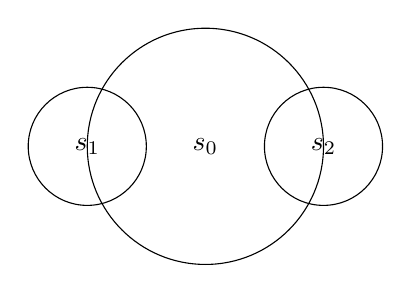
\begin{tikzpicture}[scale=0.75]
  \draw
    (0,0)
    circle
    [radius=2]
    node {$s_{0}$};
  \draw
    (-2,0)
    circle
    [radius=1]
    node {$s_{1}$};
  \draw
    (2,0)
    circle
    [radius=1]
    node {$s_{2}$};
\end{tikzpicture}
\]
Then $(\mathrm{res}_{1}(s_{0},s_{1},s_{2}))(s_{0})$ is illustrated by the three diagrams
\[
\begin{tikzpicture}[scale=0.75]
\begin{scope}
  \clip
    (0,0)
    circle
    [radius=2];
  \fill[fill=yellow]
    (-2,0)
    circle
    [radius=1];
  \clip
    (2,0)
    circle
    [radius=1];
\end{scope}
\begin{scope}
  \clip
    (7,0)
    circle
    [radius=2];
  \fill[fill=yellow]
    (9,0)
    circle
    [radius=1];
  \clip
    (5,0)
    circle
    [radius=1];
\end{scope}
  \filldraw[fill=yellow]
    (-7,0)
    circle
    [radius=2];
  \draw[pattern=dots]
    (-7,0)
    circle
    [radius=2];
  \draw
    (-9,0)
    circle
    [radius=1];
  \draw
    (-5,0)
    circle
    [radius=1];
  \draw[pattern=dots]
    (0,0)
    circle
    [radius=2];
  \draw
    (-2,0)
    circle
    [radius=1];
  \draw
    (2,0)
    circle
    [radius=1];
  \draw[pattern=dots]
    (7,0)
    circle
    [radius=2];
  \draw
    (5,0)
    circle
    [radius=1];
  \draw
    (9,0)
    circle
    [radius=1];
\end{tikzpicture}
\]
while $(\mathrm{res}_{2}(s_{0},s_{1},s_{2}))(s_{0})$ is illustrated by the three diagrams
\[
\begin{tikzpicture}[scale=0.75]
\begin{scope}
  \clip
    (0,0)
    circle
    [radius=2];
  \fill[fill=yellow]
    (-2,0)
    circle
    [radius=1];
  \clip
    (2,0)
    circle
    [radius=1];
\end{scope}
\begin{scope}
  \clip
    (7,0)
    circle
    [radius=2];
  \fill[fill=yellow]
    (9,0)
    circle
    [radius=1];
  \clip
    (5,0)
    circle
    [radius=1];
\end{scope}
  \filldraw[fill=yellow]
    (-7,0)
    circle
    [radius=2];
  \draw[pattern=dots]
    (-7,0)
    circle
    [radius=2];
  \draw
    (-9,0)
    circle
    [radius=1];
  \draw
    (-5,0)
    circle
    [radius=1];
  \draw
    (0,0)
    circle
    [radius=2];
  \draw[pattern=dots]
    (-2,0)
    circle
    [radius=1];
  \draw
    (2,0)
    circle
    [radius=1];
  \draw
    (7,0)
    circle
    [radius=2];
  \draw
    (5,0)
    circle
    [radius=1];
  \draw[pattern=dots]
    (9,0)
    circle
    [radius=1];
\end{tikzpicture}
\]
if the dotted areas correspond to the first index $k_{1}$ we fix and the second index $k_{2}$ corresponds to the three diagrams. The restriction results are always the color filled areas. We hope this illustration helps a bit. Anyways, in the end we get for a space $S$ a full subcategory
\begin{align*}
  \mathbf{Sh}(S)
\end{align*}
of
\begin{align*}
  \mathbf{Set}^{\mathbf{Open}_{S}^{\mathrm{op}}}
\end{align*}
by restricting the object set to sheaves on $\mathbf{Open}_{S}$. $\mathbf{Sh}(S)$ is called the \textbf{category of sheaves (on $S$)}
\\
Note that this definition also makes sense in other categories than $\mathbf{Set}$. The category must only have enough limits. In particular the sheaf definition makes sense for $\mathbf{C}_{\alpha}$-valued presheaves if $\mathbf{C}_{\alpha}$ is complete. In fact, $\mathbf{Grp}$-valued sheaves are common (and a few others). But one can also think of $\mathbf{Grp}$-valued sheaves as internalization (see subsection \ref{sec:internaliz}). Namely as group object (again see subsection \ref{sec:internaliz}) in $\mathbf{Sh}(S)$ since this category as topos (see subsection \ref{sec:internaliz}) has enough structure to allow these.
\\
We almost achieved our goal of formulating the second consistency condition by the descent condition. What is missing is a more general notion sensibly replacing $\mathbf{Open}_{S}$ by any category with a reasonable notion of (open) cover. Note that $\mathrm{Mor}_{\mathbf{Open}_{S}}$ has the property that
\begin{align*}
  \mathrm{i}_{U_{2}}
  \in
  \mathrm{Mor}_{\mathbf{Open}_{S}}
\end{align*}
implies that for all
\begin{align*}
  \mathrm{i}_{12}
  \in
  \mathrm{Mor}_{\mathbf{Open}_{S}}
\end{align*}
with
\begin{align*}
  \mathrm{dom}_{\mathbf{Open}_{S}}(\mathrm{i}_{U_{2}})
  &=
  \mathrm{cod}_{\mathbf{Open}_{S}}(\mathrm{i}_{12})
\end{align*}
we have
\begin{align*}
  \mathrm{i}_{U_{2}}
  \circ
  \mathrm{i}_{12}
  \in
  \mathrm{Mor}_{\mathbf{Open}_{S}}
\end{align*}
This can be interpreted as $\mathrm{i}_{U_{2}}$ punching a hole into $S$ in the form of $U_{2}$ and any $U_{1}$ smaller than $U_{2}$ fits through this hole. As a picture
\[
\begin{tikzpicture}[scale=0.25]
  \draw[pattern=grid]
    (0,0)
    circle
    [radius=8];
  \filldraw[fill=white]
    (2,0)
    circle
    [radius=4];
  \filldraw[fill=yellow]
    (2,1)
    circle
    [radius=1]
    node {\tiny{$U_{1}$}};
  \draw
    (-6,8)
    --
    (-6,8)
    node [below] {\tiny{$S$}};
  \draw
    (2,0)
    --
    (2,0)
    node [below] {\tiny{$U_{2}$}};
\end{tikzpicture}
\]
It is clear that this has to do with covers. And the idea works in general for any category since given a category $\mathbf{C}$ and an object $X$ then a subset $\mathfrak{S}_{X} \subset \mathrm{Mor}_{\mathbf{C}}$ such that
\begin{align*}
  f
  \in
  \mathfrak{S}_{X}
  \quad
  &\Rightarrow
  \quad
  \mathrm{cod}_{\mathbf{C}}(f)
  =
  X
\end{align*}
is called a \textbf{sieve (on $X$)} if
\begin{enumerate}
\item[({\#})]
for all $f \in \mathfrak{S}_{X}$ and for all $i \in \mathrm{Mor}_{\mathbf{C}}$ such that
\begin{align*}
  \mathrm{dom}_{\mathbf{C}}(f)
  &=
  \mathrm{cod}_{\mathbf{C}}(i)
\end{align*}
we have
\begin{align*}
  f
  \circ
  i
  \in
  \mathfrak{S}_{X}
\end{align*}
\end{enumerate}
It is clear that
\begin{align*}
  \mathfrak{M}_{X}
  &:=
  \bigcup_{X \in \mathrm{ob}_{\mathbf{C}}}
  \mathrm{mor}_{\mathbf{C}}(X,X_{0})
\end{align*}
is a sieve on $X_{0}$ and we call it the \textbf{maximal sieve (on $X_{0}$)}. We would still like to think of a sieve on $X$ as a cover of $X$ but we gave up on the injectivity of morphisms by this generalization which was crucial in the topological case. Hence we have to make up for this loss by demanding some properties which make the idea sufficiently close to covers. So let's see what properties we can abstract from $\mathbf{Open}_{S}$.
\begin{enumerate}
\item[(1)]
For any open subspace $U$ of $S$ we can cover $U$ by the collection of all the open subspaces of $U$. In terms of sieves we can express that by demanding the maximal sieve on $U$ to cover $U$.
\item[(2)]
Given an open subspace $U$ of $S$ which is covered by some $U_{k}$ indexed by some small set $K$ then we can clearly intersect $U$ with some other open subspace $U^{\backprime}$ of $S$ and it is clear that $U_{k} \cap U^{\backprime}$ for $k \in K$ covers $U \cap U^{\backprime}$.
\item[(3)]
Given an open subspace $U$ of $S$ which is covered by some $U_{k}$ indexed by some small set $K$ and for each $U_{k}$ a cover consisting of sets $(U_{k})_{l_{k}}$ indexed by $l_{k} \in L_{k}$ with $L_{k}$ a small set for all $k \in K$ then clearly all the $(U_{k})_{l_{k}}$ can be taken together to cover $U$.
\end{enumerate}
These ideas will yield the definition of Grothendieck topology. But we still need one last ingredient. We must somehow express the intersection in categorical terms. And here the pullback from example \ref{exa:oflimits} puts itself forward. Given a sieve $\mathfrak{S}_{X}$ and a $f \in \mathrm{Mor}_{\mathbf{C}}$ then 
\begin{align*}
  f^{\ast}(\mathfrak{S}_{X})
  &:=
  \lbrace
      h
      \in
      \mathrm{Mor}_{\mathbf{C}}
    \,
    \vert
    \,
      f
      \circ
      h
      \in
      \mathfrak{S}_{X}
  \rbrace
\end{align*}
is a sieve on $\mathrm{dom}_{\mathbf{C}}(f)$ since for $h \in f^{\ast}(\mathfrak{S}_{X})$ and all $h^{\backprime} \in \mathrm{Mor}_{\mathbf{C}}$ such that
\begin{align*}
  \mathrm{dom}_{\mathbf{C}}(h)
  &=
  \mathrm{cod}_{\mathbf{C}}(h^{\backprime})
\end{align*}
we have
\begin{align*}
  \mathrm{dom}_{\mathbf{C}}(f \circ h)
  &=
  \mathrm{cod}_{\mathbf{C}}(h^{\backprime})
\end{align*}
Thus, because $\mathfrak{S}_{X}$ containing $f \circ h$ is a sieve we can conclude
\begin{align*}
  f
  \circ
  h
  \circ
  h^{\backprime}
  &\in
  \mathfrak{S}_{X}
\end{align*}
which is to say that
\begin{align*}
  h
  \circ
  h^{\backprime}
  &\in
  f^{\ast}(\mathfrak{S}_{X})
\end{align*}
proving the claim. We then call $f^{\ast}(\mathfrak{S}_{X})$ the \textbf{pullback sieve (of $\mathfrak{S}_{X}$ along $f$)}. Indeed, it can be shown that this is actually a pullback in $\mathbf{Set}^{\mathbf{C}^{\mathrm{op}}}$. This is since sieves correspond to presheaves which can be reasonably included into representable presheaves. This inclusion is then pulled back along $\mathrm{y}_{\mathbf{C}}(f)$. Details can be found in the source we will cite in a moment. But now to Grothendieck topologies. Given a small category $\mathbf{C}$ a \textbf{Grothendieck topology (on $\mathbf{C}$)} is a function
\begin{align*}
  \mathrm{J}
  \colon
  \mathrm{ob}_{\mathbf{C}}
  &\rightarrow
  \mathrm{ob}_{\mathbf{Set}}
\end{align*}
such that each $\mathfrak{S}_{X} \in \mathrm{J}(X)$ is a sieve on $X$ for all $X$ satisfying
\begin{enumerate}
\item[(J1)]
the maximal sieve $\mathfrak{M}_{X}$ is in $\mathrm{J}(X)$ for all $X$
\item[(J2)]
if $\mathfrak{S}_{X} \in \mathrm{J}(X)$ then for any $f$ with codomain $X$ the pullback sieve $f^{\ast}(\mathfrak{S}_{X})$ is element of $\mathrm{J}(\mathrm{dom}_{\mathbf{C}}(f))$
\item[(J3)]
if $\mathfrak{S}_{X} \in \mathrm{J}(X)$ and $\mathfrak{S}_{X}^{\backprime}$ is a sieve on $X$ such that for all $f \in \mathfrak{S}_{X}$
\begin{align*}
  f^{\ast}
  \left(
    \mathfrak{S}_{X}^{\backprime}
  \right)
  &\in
  \mathrm{J}
  \left(
    \mathrm{dom}_{\mathbf{C}}(f))
  \right)
\end{align*}
then $\mathfrak{S}_{X}^{\backprime}$ is element of $\mathrm{J}(X)$.
\end{enumerate}
For a Grothendieck topology $\mathrm{J}$ we call $\mathfrak{S}_{X} \in \mathrm{J}(X)$ a \textbf{covering sieve (on $X$ w.r.t. $\mathrm{J}$)} while the pair $(\mathbf{C},\mathrm{J})$ is called a \textbf{site}.
\\
Sites are sufficient to define what it means for a presheaf on a site to be a sheaf. So assume a site $(\mathbf{C},\mathrm{J})$. Then a presheaf $P$ on $\mathbf{C}$ is a \textbf{sheaf (on $(\mathbf{C},\mathrm{J})$)} if
\begin{enumerate}
\item[(DC)]
for each object $X$ and each covering sieve $\mathfrak{S}_{X} \in \mathrm{J}(X)$ the pair $(P(X),e)$ with
\begin{align*}
  e
  \colon
  P(X)
  &\rightarrow
  \prod_{f \in \mathfrak{S}_{X}}
  P(\mathrm{dom}_{\mathbf{C}}(f))
  \\
  s
  &\mapsto
  (P(f))(s)
\end{align*}
is the equalizer of
\begin{align*}
  \mathrm{res}_{1}
  \colon
  \prod_{f \in \mathfrak{S}_{X}}
  P(\mathrm{dom}_{\mathbf{C}}(f))
  &\rightarrow
  \prod_{f \in \mathfrak{S}_{X}}
  \prod_{h \in f^{\ast}(\mathfrak{S}_{X})}
  P(\mathrm{dom}_{\mathbf{C}}(h))  
  \\
  \left(
    f
    \mapsto
    s_{f}
  \right)
  &\mapsto
  \left(
    f
    \mapsto
    \left(
      h
      \mapsto
      s_{f \circ h}
    \right)
  \right)
  \\\\
  \mathrm{res}_{2}
  \colon
  \prod_{f \in \mathfrak{S}_{X}}
  P(\mathrm{dom}_{\mathbf{C}}(f))
  &\rightarrow
  \prod_{f \in \mathfrak{S}_{X}}
  \prod_{h \in f^{\ast}(\mathfrak{S}_{X})}
  P(\mathrm{dom}_{\mathbf{C}}(h))  
  \\
  \left(
    f
    \mapsto
    s_{f}
  \right)
  &\mapsto
  \left(
    f
    \mapsto
    \left(
      h
      \mapsto
      P(h)(s_{f})
    \right)
  \right)
\end{align*}
\end{enumerate}
We refer to (DC) as \textbf{descent condition (for sheaves on $(\mathbf{C},\mathrm{J})$)} or sometimes equivalently \textbf{sheaf condition (on $(\mathbf{C},\mathrm{J})$)}. There is a site on $\mathbf{Open}_{S}$ such that the sheaf condition on that site is the sheaf condition on $\mathbf{Open}_{S}$. We have now a whole lot of possible categories of spaces. In particular there are sites on categories with objects some manifolds. This fact should make physicists prick up their ears.
\\
We have to admit here that what we have written is a bit sketchy on the motivational side. But you can convince yourself that all this is sensible by reading the first three to four chapters of the somehow worthwhile book \cite{c55c71e8}. You will then see that what we have described here is only the tip of the iceberg of some beautiful mathematics. We will mention the book again when we come to topoi in subsection \ref{sec:internaliz}.
\end{exa}
\begin{prf}
You might wish to prove here that $\Gamma_{\pi}$ is in fact a sheaf on $\mathbf{Open}_{S}$. This is essentially the topological fact that continuity is a local property and the theorem that a bunch of locally given continuous functions patch together - or better say extend here - to a unique continuous function which can be found in any topology book such as \cite{273ba834}.
\\
\phantom{proven}
\hfill
$\square$
\end{prf}
We have one last thing on limits that will be very convenient. Motivated from analysis we would like to define a sensible functor mapping functors $F$ to the apex of their (co)limiting (co)cone like one does in analysis when mapping a sequence to its limit. To this end let $F \colon \mathbf{J} \rightarrow \mathbf{C}$ be a functor with $\mathbf{J}$ small and $\mathbf{C}$ locally small. Then define the sets
\begin{align*}
  \mathrm{Lim}_{F}
  &:=
  \left\lbrace
      (X_{T},F,\mathsf{C}_{T})
      \in
      \mathrm{ob}_{(\Delta_{\mathbf{C}} \downarrow \mathrm{c}_{F})}
    \vert
      (X_{T},F,\mathsf{C}_{T})
      \text{ is a limit of }
      F
  \right\rbrace
\end{align*}
if $\mathbf{C}$ is complete and
\begin{align*}
  \mathrm{Colim}_{F}
  &:=
  \left\lbrace
      (F,X_{I},\mathsf{C}_{I}^{\prime})
      \in
      \mathrm{ob}_{(\mathrm{c}_{F} \downarrow \Delta_{\mathbf{C}})}
    \vert
      (F,X_{I},\mathsf{C}_{I}^{\prime})
      \text{ is a colimit of }
      F
  \right\rbrace
\end{align*}
if $\mathbf{C}$ is cocomplete. To achieve our goal we first need to define functions mapping functors $F$ to an element of $\mathrm{Lim}_{F}$ and $\mathrm{Colim}_{F}$, respectively. So we have to choose an element of $\mathrm{Lim}_{F}$ and $\mathrm{Colim}_{F}$, respectively, for all $F$. But the axiom of choice of TG asserts that dependent functions
\begin{align*}
  c_{\mathrm{Lim}}
  &\in
  \prod_{F \in \mathrm{ob}_{\mathbf{C}^{\mathbf{J}}}}
  \mathrm{Lim}_{F}
  \\
  c_{\mathrm{Colim}}
  &\in
  \prod_{F \in \mathrm{ob}_{\mathbf{C}^{\mathbf{J}}}}
  \mathrm{Colim}_{F}
\end{align*}
exist. To this we have an important remark.
\\
\begin{rem}
\label{rem:ordinaltrick}
Note that it is not clear that $\mathrm{Lim}_{F}$ and $\mathrm{Colim}_{F}$ are small sets and foundations such as ZFC and von Neumann-Bernays-G\"odel (abbr. NGB) lack a choice axiom powerful enough to choose from such large collections. But there is a trick with well-orders which shows how to make this still possible. The axiom of choice does only grant existence but it does not explicitly tell us what is chosen. This is actually not very nice. If, however, we constrained first-order logic to intuitionistic logic then we would have to contruct a limit/colimit explicitly to show that it exists and the axiom of choice would be superfluous here since we could define a choice function as above by just proving that the limits/colimits exist for all $F$. Hence an intuitionist does not need the axiom of choice to do the same as we do here. Indeed, in category theory it is common to work with intuitionistic logic if possible and we use the axiom of choice here only for the sake of rigor. Many authors ignore the issue due to this common practice since they think limits/colimits are constructed anyway in practice. Also note that in UFP-HoTT the issue is not really an issue since it is usually assumed intuitionistic (and all limits/colimits are formally equal by univalence). The same issue in another guise will arise for adjoints in subsection \ref{sec:adjoint} an we will refer back to this remark.
\end{rem}
\begin{prf}
The ordnial trick we addressed can be found in \cite{53fd7d7e} in chapter 7 footnote 7.
\\
\phantom{proven}
\hfill
$\square$
\end{prf}
On the whole any choice function as above yields a function mapping functors to a limit of it and the same for colimits. This function can be made into a functor as can be seen from the following discussion. So take $G_{1},G_{2} \in \mathrm{ob}_{\mathbf{C}^{\mathbf{J}}}$ and a natural transformation $\mathsf{T} \colon G_{1} \Rightarrow G_{2}$.
\begin{align*}
  \left(
    X_{T}^{k},
    G_{k},
    \mathsf{C}_{T}^{k}
  \right)
\end{align*}
shall denote a limiting cone to $G_{k}$ with apex $X_{T}^{k}$ for $k = 1,2$. Then there is a unique morphism
\begin{align*}
  \mathsf{T}_{!}
  &\in
  \mathrm{mor}_{\mathbf{C}}
  \left(
    X_{T}^{1},
    X_{T}^{2}
  \right)
\end{align*}
determined by the commutative diagram
\[
\begin{tikzcd}[row sep=huge, column sep=9em]
  G_{1}(J_{1})
  \arrow{rr}{G_{1}(j_{12})}
  \arrow[swap]{ddd}{\mathsf{T}(J_{1})}
  &
  &
  G_{1}(J_{2})
  \arrow{ddd}{\mathsf{T}(J_{2})}
  \\
  &
  X_{T}^{1}
  \arrow{ur}{\mathsf{C}_{T}^{1}(J_{2})}
  \arrow[dashed]{d}{\mathsf{T}_{!}}
  \arrow[swap]{ul}{\mathsf{C}_{T}^{1}(J_{1})}
  &
  \\
  &
  X_{T}^{2}
  \arrow[swap]{dr}{\mathsf{C}_{T}^{2}(J_{2})}
  \arrow{dl}{\mathsf{C}_{T}^{2}(J_{1})}
  &
  \\
  G_{2}(J_{1})
  \arrow{rr}{G_{2}(j_{12})}
  &
  &
  G_{2}(J_{2})
\end{tikzcd}
\]
This works since $\mathsf{T} \circ \mathsf{C}_{T}^{1}$ is a cone to $G_{2}$ with apex $X_{T}^{1}$. Dually, let
\begin{align*}
  \left(
    G_{k},
    X_{I}^{k},
    \mathsf{C}_{I}^{k}
  \right)
\end{align*}
denote a colimiting cocone to $G_{k}$ with apex $X_{I}^{k}$ for $k = 1,2$. Then there is a unique morphism
\begin{align*}
  \mathsf{T}_{!}^{\prime}
  &\in
  \mathrm{mor}_{\mathbf{C}}
  \left(
    X_{I}^{1},
    X_{I}^{2}
  \right)
\end{align*}
determined by the commutative diagram
\[
\begin{tikzcd}[row sep=huge, column sep=9em]
  G_{1}(J_{1})
  \arrow{rr}{G_{1}(j_{12})}
  \arrow[swap]{ddd}{\mathsf{T}(J_{1})}
  \arrow{dr}{\mathsf{C}_{I}^{1}(J_{1})}
  &
  &
  G_{1}(J_{2})
  \arrow[swap]{dl}{\mathsf{C}_{I}^{1}(J_{2})}
  \arrow{ddd}{\mathsf{T}(J_{2})}
  \\
  &
  X_{I}^{1}
  \arrow[dashed]{d}{\mathsf{T}_{!}^{\prime}}
  &
  \\
  &
  X_{I}^{2}
  &
  \\
  G_{2}(J_{1})
  \arrow[swap]{ur}{\mathsf{C}_{I}^{2}(J_{1})}
  \arrow{rr}{G_{2}(j_{12})}
  &
  &
  G_{2}(J_{2})
  \arrow{ul}{\mathsf{C}_{I}^{2}(J_{2})}
\end{tikzcd}
\]
This works again since $\mathsf{C}_{I}^{2} \circ \mathsf{T}$ is a cocone to $G_{1}$ with apex $X_{I}^{2}$. Now we are sufficiently prepared to define the functors. Given the choice functions $c_{\mathrm{Lim}}$ and $c_{\mathrm{Colim}}$ we can define functors
\begin{align*}
  \varprojlim_{\mathbf{J}}
  \doteq
  \varprojlim_{\mathbf{J}}^{c_{\mathrm{Lim}}}
  \colon
  \mathbf{C}^{\mathbf{J}}
  &\rightarrow
  \mathbf{C}
  \\
  F
  &\mapsto
  \mathrm{pr}_{1}
  \circ
  c_{\mathrm{Lim}}(F)
  \\
  \mathsf{T}
  &\mapsto
  \mathsf{T}_{!}
  \\
  \\
  \varinjlim_{\mathbf{J}}
  \doteq
  \varinjlim_{\mathbf{J}}^{c_{\mathrm{Colim}}}
  \colon
  \mathbf{C}^{\mathbf{J}}
  &\rightarrow
  \mathbf{C}
  \\
  F
  &\mapsto
  \mathrm{pr}_{2}
  \circ
  c_{\mathrm{colim}}(F)
  \\
  \mathsf{T}
  &\mapsto
  \mathsf{T}_{!}^{\prime}
\end{align*}
$\varprojlim_{\mathbf{J}}^{c_{\mathrm{Lim}}}$ is called \textbf{limit functor (for $c_{\mathrm{Lim}}$ over $\mathbf{J}$)} while $\varinjlim_{\mathbf{J}}^{c_{\mathrm{Colim}}}$ is called \textbf{colimit functor (for $c_{\mathrm{colim}}$ over $\mathbf{J}$)}. The convention is that the choice functions $c_{\mathrm{Lim}}$ and $c_{\mathrm{Colim}}$ are silently assumed to be the canonical ones obtained from constructing the limits explicitly if possible (which is practically always possible in category theory) and else the choice functions obtained from the axiom of choice when technically necessary. Again, it is common not to mention them in practice and so will we do in the following. As a last remark here, limit and colimit functors for different choice functions are naturally isomorphic as is apparent essentially from theorem \ref{thm:uniqueuniarr} which implies that limits are unique up to unique isomorphism. So structurally the choice function is not essential.
\\\\
We are now able to prove the last fact about bicompleteness we need. It is that functor categories are bicomplete if the codomain category is.
\\
\begin{thm}
\label{thm:funccatbicomplete}
Let $\mathbf{C}$ be small.
\begin{enumerate}
\item[(1T)]
If $\mathbf{C}_{\alpha}$ is complete then so is $\mathbf{C}_{\alpha}^{\mathbf{C}}$.
\item[(1I)]
If $\mathbf{C}_{\alpha}$ is cocomplete then so is $\mathbf{C}_{\alpha}^{\mathbf{C}}$.
\end{enumerate}
\end{thm}
\begin{prf}
\begin{enumerate}
\item[(1T)]
Let
\begin{align*}
  F
  \colon
  \mathbf{J}
  &\rightarrow
  \mathbf{C}_{\alpha}^{\mathbf{C}}
\end{align*}
be a functor. By premise, we have a limiting cone $\mathsf{C}_{T}^{X}$ to $(F(\cdot))(X)$ with apex
\begin{align*}
  \varprojlim_{\mathbf{J}}
  \left(
    (F(\cdot))(X)
  \right)
\end{align*}
and we can define a functor
\begin{align*}
  \varprojlim^{F}
  \colon
  \mathbf{C}
  &\rightarrow
  \mathbf{C}_{\alpha}
  \\
  X
  &\mapsto
  \varprojlim_{\mathbf{J}}
  \left(
    (F(\cdot))(X)
  \right)
  \\
  f_{12}
  &\mapsto
  \varprojlim_{\mathbf{J}}
  \left(
    (F(\cdot))(f_{12})
  \right)
\end{align*}
Hence we can define a cone $\mathsf{C}_{T}$ to $F$ by mapping $J$ to the natural transformation
\begin{align*}
  \mathsf{C}_{T}(J)
  \colon
  \varprojlim^{F}
  &\Rightarrow
  F(J)
  \\
  X
  &\mapsto
  \mathsf{C}_{T}^{X}(J)
\end{align*}
Once more we proceed in two steps to finish the proof.
\begin{description}
\item[Step 1]
$\mathsf{C}_{T}$ is in fact a cone since
\begin{align*}
  \left(
    F(j_{12})
    \circ
    \mathsf{C}_{T}(J_{1})
  \right)
  (X)
  &=
  (F(j_{12}))(X)
  \circ
  \left(
    \mathsf{C}_{T}(J_{1})
  \right)
  (X)
  \\
  &=
  (F(j_{12}))(X)
  \circ
  \mathsf{C}_{T}^{X}(J_{1})
  \\
  &=
  \mathsf{C}_{T}^{X}(J_{2})
  \\
  &=
  \left(
    \mathsf{C}_{T}(J_{2})
  \right)
  (X)
\end{align*}
for all $j_{12}$ and $X$.
\item[Step 2]
$\mathsf{C}_{T}$ is also limiting since for any cone $\mathsf{C}$ to $F$ with apex $G \colon \mathbf{C} \rightarrow \mathbf{C}_{\alpha}$ we have that $(\mathsf{C}(\cdot))(X)$ is a cone to $(F(\cdot))(X)$ for all $X$ and by premise there is a unique
\begin{align*}
  \mathsf{C}_{!}^{X}
  \in
  \mathrm{mor}_{\mathbf{C}_{\alpha}}
  \left(
    G(X),
    \varprojlim^{F}(X)
  \right)
\end{align*}
such that
\begin{align*}
  \mathsf{C}_{T}^{X}(J)
  \circ
  \mathsf{C}_{!}^{X}
  &=
  (\mathsf{C}(J))(X)
\end{align*}
for all $J$. Hence the natural transformation
\begin{align*}
  \mathsf{C}_{!}
  \colon
  G
  &\Rightarrow
  \varprojlim^{F}
  \\
  X
  &\mapsto
  \mathsf{C}_{!}^{X}
\end{align*}
is the unique morphism such that
\begin{align*}
  \left(
    \mathsf{C}_{T}(J)
    \circ
    \mathsf{C}_{!}
  \right)
  (X)
  &=
  \left(
    \mathsf{C}_{T}(J)
  \right)
  (X)
  \circ
  \mathsf{C}_{!}(X)
  \\
  &=
  \mathsf{C}_{T}^{X}(J)
  \circ
  \mathsf{C}_{!}^{X}
  \\
  &=
  (\mathsf{C}(J))(X)
\end{align*}
\end{description}
\item[(1I)]
The duality principle \ref{thm:dp}.
\end{enumerate}
\phantom{proven}
\hfill
$\square$
\end{prf}
Hence in the case of completeness limits are computed {\glqq}pointwise{\grqq} and so are colimits in case of cocompleteness. But if we are not complete or cocomplete this is not necessarily the case. 
